\documentclass[a4paper,11pt]{article}
\usepackage[utf8]{inputenc}
\usepackage{amsmath}
\usepackage{amsfonts}
\usepackage[top=1in, bottom=1in, left=1in, right=1in]{geometry}
\usepackage{graphicx}
\usepackage{lastpage}
\usepackage{fancyhdr}
\usepackage{xcolor}
\usepackage[english]{babel}
\usepackage[parfill]{parskip}
\usepackage{listings}
\usepackage{hyperref}
\usepackage{titlesec}
\usepackage{float}
\usepackage{tikz}
\usetikzlibrary{automata, positioning}
\begin{document}

\section*{Solutions exercises Queuing Theory and Simulation}

\textbf{Go to \url{https://github.com/Anton-4/queuing-exercises} to get the most recent version of this document}

I found that the solutions written down in class often missed steps, important details and explanations, which is why I have created this document with detailed,
annotated and complete solutions for most exercises.

If certain solutions are unclear or new exercises are given please create issues or contribute to the github repository so that we can maintain this document over the years.

This document was based on notes by ir. Mathias De Brouwer and ir. Anton Van Moere, \LaTeX created by Anton Van Moere.
Help in understanding and expanding solutions was provided by ir. Alexander Erreygers and dr. Sarah Dendievel.
Course was given by Professor Dieter Fiems and Professor. ir. Joris Walraevens.

\section{ Probability refresher }

\subsection*{1.}

\textbf{used formulas}

mean discrete function $= E[g(X)]= \sum_{i=1}^n g(i)\cdot Pr[X=i]$

\textbf{solution}

N = number of students in  avg class, with N a random variable\\
mean = $E[N]=20$\\
\\
for our example, a class has either 2 or 100 students
$N-\mathcal{N}=\{2,100\}$\\

\begin{align*}
E[N]&=2\cdot Pr(N=2)+100\cdot Pr(N=100)\\
&=2\cdot Pr(N=2)+100\cdot (1-Pr(N=2))\\
&=100-98\cdot Pr(N=2)\\
\end{align*}

$\Rightarrow Pr(N=2)=\frac{80}{98},Pr(N=100)=\frac{18}{98}$\\
\\
$\widetilde{N}=$ nr students in class of randomly selected student\\
\\
$Pr(\widetilde{N}=100)=\frac{100\cdot Pr[N=100]}{\sum_{i}i\cdot Pr[N=i]}=\frac{18\cdot 100}{18\cdot 100+80\cdot 2}=\frac{1800}{1960}=0.918$\\
\\
$\Rightarrow$ Dean is right

\subsection*{2.}

\textbf{used formulas}

\begin{align*}
E[a\cdot X] &=a\cdot E[X]\\
Var[X] &= E[(X-E[X])^{2}] = E[X^2] - E[X]^2\\
E[X + Y] &= E[X] + E[Y]\\
V,W:Var[V+W] &= Var[V]+Var[W]\text{, if independent}\\
\end{align*}

\textbf{solution}

capital $c\in\mathbb{N}$
interest first strategy: $y_{1}=c\cdot X$\\

\begin{align*}
  E[y_{1}]=E[c\cdot X]\\
  =c\cdot E[X]
\end{align*}

\begin{align*}
Var[y_{1}]&=Var[c\cdot X]\\
&=E[(cX-E[cX])^{2}]\\
&=E[(c\cdot X)^{2}]-(E[c\cdot X])^{2}\\
&=c^2 E[X^2]-(c\cdot E[X])^{2}\\
&=c^{2}Var[X]
\end{align*}

interest second strategy: $y_{2}=\sum_{{i=1}}^{c}X_{i}$\\
\\
\begin{align*}
E[y_{2}]&=E[\sum_{{i=1}}^{c}X_{i}]\\
&=\sum_{{i=1}}^{c}E[X_{i}]\\
&=c\cdot E[X]\\
\end{align*}
\\
\begin{align*}
Var[y_{2}]&=Var[\sum_{{i=1}}^{c}X_{i}]\\
&=\sum_{{i=1}}^{c}Var[X_{i}]\\
&=c\cdot Var[X]\\
\end{align*}
\\
$\Rightarrow$ the second strategy is less risky because of lower variance

\subsection*{ 3. }

\textbf{used formulas}

\begin{align*}
E[g(X)] &= \sum_{i=1}^n g(i)\cdot Pr[X=i]\\
E\left[X \cdot Y\right] &= E\left[X\right]\cdot E\left[Y\right]
\end{align*}
\clearpage
\textbf{solution}

to prove or disprove: $E\left[\frac{A}{B}\right]=\frac{E\left[A\right]}{E\left[B\right]}$

\begin{align*}
A:A\subset \mathbb{Z}\\
B:B\subset \mathbb{Z}\backslash\{0\}\\
E\left[B\right]\ne 0
\end{align*}

\begin{align*}
E\left[\frac{A}{B}\right]&=\sum_{{a\in A}}\sum_{{b\in B}}\frac{a}{b}Pr\left[A=a,B=b\right]\\
&=\sum_{{a\in A}}\sum_{{b\in B}}\frac{a}{b}Pr\left[A=a\right]\cdot Pr\left[B=b\right]&& \text{- joint of independent vars -}
\end{align*}

\begin{align*}
\frac{E\left[A\right]}{E\left[B\right]}&=\frac{\sum_{{a\in A}}a\cdot Pr\left[A=a\right]}{\sum_{{b\in B}}b\cdot Pr\left[B=b\right]}
\end{align*}

the above equations are clearly not equal

\subsection*{4. }

\textbf{used formulas}

Properties exponential distribution:
\begin{align*}
\text{distribution function = } F\left(x\right)&=1-\exp\left(-\lambda\cdot x\right)\\
\text{density function = } f\left(x\right)&=\frac{d}{dx}F\left(x\right)=\lambda\cdot \exp\left(-\lambda\cdot x\right)\\
\text{mean = } E\left[X\right]&=\int_{0}^{{+\infty}}x\cdot f\left(x\right)dx=\int_{0}^{\infty}x\cdot \lambda\cdot \exp\left(-\lambda\cdot x\right)=\frac{1}{\lambda}
\end{align*}

\begin{align*}
F\prime \left(t\right) &= \frac{F\left(t+\delta \right)-F\left(t\right)}{\delta }\\
Pr\left[A|B\right]&=\frac{Pr\left[B|A\right]\cdot Pr\left[A\right]}{Pr\left[B\right]}\\
&=\frac{Pr\left[A\cap B\right]}{Pr\left[B\right]}\\
F(t) &= Pr[X \le t]
\end{align*}

property mean r.v.

$Y=$ positive continuous random var $\rightarrow$ $\forall y< 0|f_{Y}\left(y\right)=0$
\begin{align*}
E\left[Y\right]&=\int _{0}^{\infty }yf_{Y}\left(y\right)dy&& \\\text{-  mean continuous r.v. -}
\text{integration by parts: $\int u \cdot dv = u \cdot v - \int v \cdot du$}\\
\text{$u = y, du = dy, dv = f_y(y)dy, v = F_y(y)-1$}\\
&=y\left(F_{Y}\left(y\right)-1\right)\bigg\rvert _{0}^{\infty }-\int _{0}^{\infty }\left(F_{y}\left(y\right)-1\right)dy&& \\\text{- integral of density is cdf -}\\
&=\int _{0}^{\infty }\left(1-F_{y}\left(y\right)\right)dy&& \text{-  $F_{Y}\left(\infty \right)=1$ -}
\end{align*}

\textbf{solution}

\textbf{given:}

distribution F(t) of the hard drive lifetime X is a mixture of exponentials:
\begin{align*}
F\left(t\right)&=Pr\left[X\le t\right]=p\cdot \left(1-\exp\left(-\lambda_{1}\cdot t\right)\right)+\left(1-p\right)\cdot \left(1-\exp\left(-\lambda_{2}\cdot t\right)\right)\\
&=1-p\cdot \exp\left(-\lambda_{1}\cdot t\right)-\left(1-p\right)\cdot \exp\left(-\lambda_{2}\cdot t\right)
\end{align*}
The first exponential represents probability of failure during production,
the second is prob of failure during normal use.

\begin{align*}
p&=0.1\\
\lambda_{1}&=10\\
\lambda_{2}&=1
\end{align*}

\subsubsection*{ a) }

failure rate $=\lambda \left(t\right)=\frac{F\sp{\prime} \left(t\right)}{1-F\left(t\right)}$
\begin{align*}
\frac{F\sp{\prime} \left(t\right)}{1-F\left(t\right)}&=\frac{1}{1-F\left(t\right)}\cdot F\prime \left(t\right)\\
&=\frac{1}{1-F\left(t\right)}\cdot \frac{F\left(t+\delta \right)-F\left(t\right)}{\delta }&& \text{-  formule afgeleide -}\\
&=\frac{1}{1-Pr\left[T\le t\right]}\cdot \frac{F\left(t+\delta \right)-F\left(t\right)}{\delta }&& \text{-  $F\left(t\right)=Pr\left[T\le t\right]$ -}\\
&=\frac{1}{Pr\left[T> t\right]}\cdot \frac{Pr\left[T\le t+\delta \right]-Pr\left[T\le t\right]}{\delta }&& \text{-  $F\left(x\right)=Pr\left[T\le x\right]$ -}\\
&=\frac{Pr\left[t< T,T\le t+\delta \right]}{Pr\left[T> t\right]\cdot \delta }\\
&=\frac{Pr\left[T\le t+\delta |T> t\right]}{\delta }&& \text{-  bayes rule -}
\end{align*}

$\lambda \left(t\right)$ = probability it will fail at time $t+dt$ given it has not failed until time t

\subsubsection*{ b) }

remaining lifetime $=X_{R}=X-t$

\begin{align*}
F_{{X_{R}}}\left(x|t\right)&=Pr\left[X_{R}\le x|X> t\right]&& \text{-  property cdf -}\\
&=Pr\left[X-t\le x|X> t\right]&& \text{-  $X_{R}=X-t$ -}\\
&=\frac{Pr\left[X\le x+t,X> t\right]}{Pr\left[X> t\right]}&& \text{-  bayes rule -}\\
&=\frac{F\left(x+t\right)-F\left(t\right)}{1-F\left(t\right)}&& \text{-  property cdf -}\\
&=\frac{F\left(x+t\right)+\left(1-F\left(t\right)\right)-1}{1-F\left(t\right)}\\
&=1-\frac{1-F\left(x+t\right)}{1-F\left(t\right)}\\
&=1-\frac{p\cdot \exp \left(-\lambda _{1}\cdot \left(t+x\right)\right)+\left(1-p\right)\cdot \exp \left(-\lambda _{2}\cdot \left(t+x\right)\right)}{p\cdot \exp \left(-\lambda _{1}\cdot t\right)+\left(1-p\right)\cdot \exp \left(-\lambda _{2}\cdot t\right)}&& \text{-  fill in from given -}
\end{align*}

\subsubsection*{c) }

asked: mean of remaining life time =
\begin{align*}
E\left[X_{R}|X> t\right]&=\int _{0}^{\infty }x\cdot dF_{{X_{R}}}\left(x|t\right)\\
&=\int _{0}^{\infty }\left(1-F_{{X_{R}}}\left(x|t\right)\right)dx&& \text{-  see property mean r.v. -}\\
&=\ldots \\
&=\frac{1}{\lambda _{1}\cdot \lambda _{2}}\cdot \frac{p\cdot \lambda _{2}\cdot \exp \left(-\lambda _{1}\cdot t\right)+\left(1-p\right)\cdot \lambda _{1}\cdot \exp \left(-\lambda _{2}\cdot t\right)}{p\cdot \exp \left(-\lambda _{1}\cdot t\right)+\left(1-p\right)\cdot \exp \left(-\lambda _{2}\cdot t\right)}
\end{align*}

lifetime increases when using it more (counterintuitive but true)

\clearpage

\subsection*{ 5. }

\textbf{used formulas}

\begin{align*}
E\left[X\right]&=E\left[E\left[X|Y\right]\right]
\end{align*}

\textbf{solution}

S = file size

average file size =  E[S] = 6K

\subsubsection*{ a) }
\textbf{to prove:} fewer than half of the files can have size \textgreater  12K

\begin{align*}
E\left[S\right]&=E\left[E\left[S|X\right]\right]&& \text{-  property conditional expectation -}\\
&=E\left[S|S> 12K\right]\cdot Pr\left[S> 12K\right]+E\left[S|S\le 12K\right]\cdot Pr\left[S\le 12K\right]&& \text{-  def expectation -}\\
&=E\left[S|S> 12K\right]\cdot Pr\left[S> 12K\right]+E\left[S|S\le 12K\right]\cdot \left(1-Pr\left[S> 12K\right]\right)\\
6K&=\left(E\left[S\right]> 12K\right)\cdot Pr\left[S> 12K\right]+0\cdot \left(1-Pr\left[S> 12K\right]\right)&& \text{-  take lower bound -}
\end{align*}
$\implies$ $\frac{1}{2}> Pr\left[S> 12K\right]$

\subsubsection*{ b) }
min file size is 3K, max amount of \textgreater 12K files
\begin{align*}
6> 12\cdot Pr\left[S> 12K\right]+3\cdot \left(1-Pr\left[S> 12K\right]\right)\\
\frac{1}{3}> Pr\left[S> 12K\right]
\end{align*}

\subsection*{ 6. }

\textbf{used formulas}

\begin{align*}
Pr\left[X+Y\le t\right] &=\int _{{-\infty }}^{{+\infty }}Pr\left[X\le t-y\right]dF_{Y}\left(y\right) && \text{- see A.1.5 -}
\end{align*}

\textbf{solution}

company pays fine if processing time exceeds 7 seconds

retrieving file takes time X exponentially distributed with mean 5

parsing file takes time Y uniformly distributed over [1, 3]

$T=X+Y> 7$

\begin{align*}
Pr\left[T> 7\right]&=1-Pr\left[T\le 7\right]\\
&=1-F_{T}\left(7\right)&& \text{-  property cdf -}
\end{align*}

\begin{align*}
F_{T}\left(t\right)&=Pr\left[T\le t\right]\\
&=Pr\left[X+Y\le t\right]\\
&=\int _{{-\infty }}^{{+\infty }}Pr\left[X\le t-y\right]dF_{Y}\left(y\right)&& \text{- see formulas -}
\end{align*}
$X$ is exponentially distributed, so based on table 1 at A.1.11:
\begin{align*}
F_{X}\left(x\right)&=1-\exp \left(-\lambda \cdot t\right)\\
E\left[X\right]&=5=\frac{1}{\lambda }
\end{align*}
$Y$ is uniformly distributed, so based on table 1:
\begin{align*}
F_{y}\left(y\right)&=\begin{cases}
0&y< 1\\
\frac{1}{2}\left(y-1\right)&1\le y\le 3\\
1&y> 3\\
\end{cases}
\end{align*}

\begin{align*}
f_{Y}\left(y\right)&=\begin{cases}
0&y< 1\\
\frac{1}{2}&1\le y\le 3\\
0&y> 3\\
\end{cases}
\end{align*}

We set boundaries to 1 and 3 because $f_Y(y) = 0$ everywhere else
\begin{align*}
F_{T}\left(t\right)&=\int _{1}^{3}F_{X}\left(t-y\right)f_{Y}\left(y\right)dy\\
&=\int _{1}^{3}(1-e^{-\lambda \cdot \left(t-y\right)}) \frac{1}{2} dy\\
&=\frac{1}{2} \int _{1}^{3}1-e^{-\lambda \cdot \left(t-y\right)} dy\\
&=\frac{1}{2} \int _{1}^{3}1 - \frac{1}{2} \int _{1}^{3} e^{-\lambda \cdot \left(t-y\right)} dy\\
&=\frac{1}{2} \cdot 2 - \frac{1}{2} \int _{1}^{3} e^{-\lambda t}\cdot e^{\lambda y} dy\\
&= 1 - \frac{1}{2} \int _{1}^{3} e^{-\lambda t}\cdot e^{\lambda y} dy\\
&= 1 - \frac{1}{2} e^{-\lambda t} \int _{1}^{3} e^{\lambda y} dy\\
&= 1 - \frac{1}{2} e^{-\lambda t} \left[ -\frac{e^{\lambda y}}{\lambda} \right]_1^3\\
&= 1 - \frac{e^{-\lambda t}}{2} \cdot \left(\frac{e^{-\lambda 3}}{\lambda} -\frac{e^{\lambda}}{\lambda}\right)\\
&=1-\frac{e^{{-\lambda t}}}{2\cdot \lambda }\left(e^{{\lambda 3}}-e^{\lambda }\right)
\end{align*}
\begin{align*}
Pr\left[T> 7\right]&=1-Pr\left[T\le 7\right]\\
&= 1-\frac{e^{{-0.2 \cdot 7}}}{2\cdot 0.2 }\left(e^{{0.2 \cdot 3}}-e^{0.2 }\right) \\
&=0.3703
\end{align*}

\subsection*{ 7. }

if  $Pr\left[A|B\right]> Pr\left[A\right]$ , prove that:  $Pr\left[B|A\right]> Pr\left[B\right]$

\begin{align*}
Pr\left[A\right]&< Pr\left[A|B\right]\\
Pr\left[A\right]&< \frac{Pr\left[A\cap B\right]}{Pr\left[B\right]}&& \text{-  bayes theorem -}
\end{align*}
\begin{align*}
\text{assume that }Pr\left[A\right]> 0,Pr\left[B\right]> 0
\end{align*}
\begin{align*}
Pr\left[B\right]&< \frac{Pr\left[A\cap B\right]}{Pr\left[A\right]}\\
Pr\left[B\right]&< Pr\left[B|A\right]&& \text{-  bayes theorem -}
\end{align*}

\subsection*{ 8. }

\textbf{used formulas}

\begin{align*}
E\left[X|Y=y\right]&=\sum _{{i=1}}^{\infty} Pr[X = i| Y = y] \cdot i\\
\sum _{{n=1}}^{\infty}n\cdot z^{n}&=\frac{z}{\left(1-z\right)^{2}}\\
\sum _{{n=1}}^{\infty}n^{2}z^{n} &= \frac{z\left(1+z\right)}{\left(1-z\right)^{3}}
\end{align*}

\textbf{solution}

95\% good chips, 5\% bad chips\\
good chips will fail with probability 0.0001 each day\\
bad chips will fail with probability 0.01 each day\\
time until chip fails =  T\\
compute $E\left[T\right]$ and $var\left[T\right]$

state of random chip =  $S=\{g,b\}$
\begin{align*}
Pr\left[S=g\right]&=0.95\\
Pr\left[S=b\right]&=0.05\\
Pr\left[fail|S=g\right]&=0.0001=p_{g}\\
Pr\left[fail|S=b\right]&=0.01=p_{b}
\end{align*}

\begin{align*}
E\left[T\right]&=E\left[E\left[T|S\right]\right]=Pr\left[S=g\right]\cdot E\left[T|S=g\right]+Pr\left[S=b\right]\cdot E\left[T|S=b\right]
\end{align*}

\begin{align*}
Pr\left[T=1|S=g\right]&=0.0001\\
Pr\left[T=2|S=g\right]&=\left(1-Pr\left[fail|S=g\right]\right)\cdot Pr\left[fail|S=g\right]\\
Pr\left[T=n|S=g\right]&=\left(1-Pr\left[fail|S=g\right]\right)^{\left(n-1\right)}\cdot Pr\left[fail|S=g\right]\\
&=\left(1-p_{g}\right)^{\left(n-1\right)}\cdot p_{g}
\end{align*}

\begin{align*}
E\left[T|S=g\right]&=\sum _{{n=1}}^{\infty}\left(1-p_{g}\right)^{\left(n-1\right)}\cdot p_{g}\cdot n && \text{multiplied by n because we want to sum time, not probabilities}
\end{align*}

\begin{align*}
E\left[T|S=g\right]&=\sum _{{n=1}}^{\infty}\left(1-p_{g}\right)^{{n-1}}\cdot p_{g}\cdot n\\
&=\frac{p_{g}}{1-p_{g}}\cdot \sum _{{n=1}}^{\infty}n\cdot \left(1-p_{g}\right)^{n} \text{-  prop geom series -}\\ 
&=\frac{p_{g}}{1-p_{g}}\cdot \frac{1-p_{g}}{p_{g}^{2}}\\
&=\frac{1}{p_g}
\end{align*}
\begin{align*}
E\left[T|S=b\right]&=\frac{1}{p_{b}}
\end{align*}

$=> E\left[T\right]=0.95\cdot \frac{1}{p_{g}}+0.05\cdot \frac{1}{p_{b}}=9505$ days

\begin{align*}
Var\left[T\right]&=E\left[\left(T-E\left(T\right)\right)^{2}\right]\\
&=E\left[T^{2}\right]-\left(E\left[T\right]\right)^{2}
\end{align*}
\begin{align*}
E\left[T^{2}\right]&=E\left[T^{2}|S=g\right]\cdot Pr\left[S=g\right]+E\left[T^{2}|S=b\right]\cdot Pr\left[S=b\right]
\end{align*}


\begin{align*}
Pr\left[T^{2}=1|S=g\right]&=Pr\left[T=1|S=g\right]=p_{g}\\
Pr\left[T^{2}=4|S=g\right]&=Pr\left[T=2|S=g\right]=\left(1-p_{g}\right)p_{g}\\
Pr\left[T^{2}=n^{2}|S=g\right]&=Pr\left[T=n|S=g\right]=\left(1-p_{g}\right)^{\left(n-1\right)}\cdot p_{g}
\end{align*}
\begin{align*}
E\left[T^{2}|S=g\right]&=\sum _{{n=1}}^{\infty }n^{2}\left(1-p_{g}\right)^{\left(n-1\right)}p_{g}\\
&=\frac{p_{g}}{1-p_{g}}\cdot \sum _{{n=1}}^{\infty }n^{2}\left(1-p_{g}\right)^{n}\\
&=\frac{p_{g}}{1-p_{g}}\cdot \frac{\left(1-p_{g}\right)\left(2-p_{g}\right)}{p_{g}^{3}}&& \text{-  see formulas -}\\
&=\frac{2-p_{g}}{p_{g}^{2}}
\end{align*}

\begin{align*}
E\left[T^{2}\right]&=0.95\cdot \frac{2-p_{g}}{p_{g}^{2}}+0.05\frac{2-p_{b}}{p_{b}^{2}}
\end{align*}

\begin{align*}
Var\left[T\right] &= E\left[T^{2}\right]-\left(E\left[T\right]\right)^{2}\\
&= 0.95\cdot \frac{2-p_{g}}{p_{g}^{2}}+0.05\frac{2-p_{b}}{p_{b}^{2}} - 9505^2\\
&= 99,646,470 \\
std &= 9982.3 \text{ days}
\end{align*}

properties geometric series:
\begin{align*}
\sum _{{n=0}}^{\infty}z^{n}&=\frac{1}{1-z}&& \text{-  if $|z|< 1$ -}\\
\sum _{{n=1}}^{\infty}n\cdot z^{n}&=z\cdot \sum _{{n=1}}^{\infty}n\cdot z^{{n-1}}=z\sum _{{n=1}}^{\infty}\frac{d}{dz}z^{n}=z\frac{d}{dz}\left(\sum _{{n=0}}^{\infty}z^{n}\right)\\
&=z\cdot \frac{d}{dz}\left(\frac{1}{1-z}\right)=z\cdot \frac{\left(-1\right)^{2}}{\left(1-z\right)^{2}}=\frac{z}{\left(1-z\right)^{2}}
\end{align*}
\begin{align*}
\sum _{{n=1}}^{\infty}n^{2}z^{n}&=z\cdot \sum _{{n=1}}^{\infty}n^{2}z^{\left(n-1\right)}\\
&=z\cdot \sum _{{n=1}}^{\infty}\frac{d}{dz}\left(n\cdot z^{n}\right)\\
&=z\cdot \frac{d}{dz}\left(\sum _{{n=0}}^{\infty}n\cdot z^{n}\right)\\
&=z\cdot \frac{\left(1-z\right)^{2}+2\cdot \left(1-z\right)\left(-1\right)}{\left(1-z\right)^{4}}\\
&=\frac{z\left(1+z\right)}{\left(1-z\right)^{3}}
\end{align*}

\clearpage

\section{Markov chains}

\subsection*{ 1. }

$p_{{i,j}}=Pr\left[W_{{n+1}}=j|W_{n}=i\right]$

webpages =  $W=\{1,2,3\}$

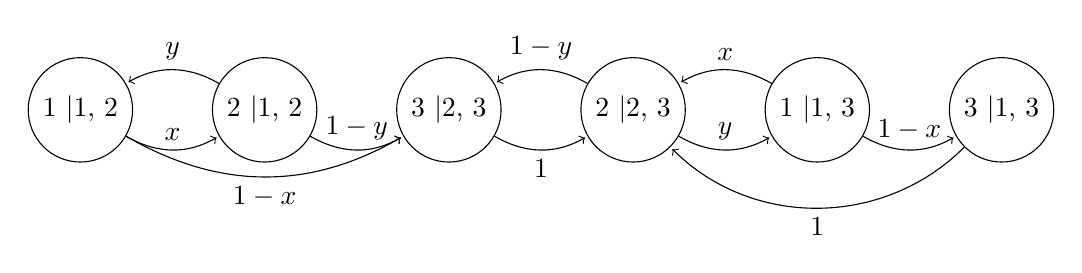
\begin{tikzpicture}
        \node[state]             (0) {3 \textbar 2, 3};
        \node[state, right=of 0] (1) {2 \textbar 2, 3};
        \node[state, right=of 1] (2) {1 \textbar 1, 3};
        \node[state, right=of 2] (3) {3 \textbar 1, 3};
        \node[state, left=of 0] (4) {2 \textbar 1, 2};
        \node[state, left=of 4] (5) {1 \textbar 1, 2};

        \draw[every loop]
            (0) edge[bend right, auto=right]  node {1} (1)
            (1) edge[bend right, auto=right] node {$1 - y$} (0)
            (1) edge[bend right, auto=right, above]  node {$y$} (2)
            (2) edge[bend right, auto=right] node {$x$} (1)
            (2) edge[bend right, auto=right, above]  node {$1-x$} (3)
            (3) edge[bend left=45, auto=right, below] node {$1$} (1)
            (4) edge[bend right, auto=right]  node {$y$} (5)
            (4) edge[bend right, auto=right, above]  node {$1 - y$} (0)
            (5) edge[bend right, auto=right, above] node {$x$} (4)
            (5) edge[bend right, auto=right] node {$1 - x$} (0)
            ;
\end{tikzpicture}

proportion of time cache contains pages $k+l=t_{{k,l}}$

\textbf{Ergodic?}
\begin{itemize}
\item  finite state space W? $\rightarrow$ yes
\item  gcd\{2,3,4,5,...\} = 1 for all sates $\rightarrow$  aperiodic
\item  irriducible? - yes
\item \textgreater  Markov chain is ergodic  $\rightarrow$  limiting distribution = stationary distribution
\end{itemize}

transient state = time spent in state is 0 in the long run

$t_{{1,2}}=0$, since it is a transient state

transient states can be removed, stationary equations:

\begin{align*}
\pi _{{\left(3,2,3\right)}}&=\pi _{{\left(2,2,3\right)}}\cdot \left(1-y\right)\\
\pi _{{\left(2,2,3\right)}}&=\pi _{{\left(3,2,3\right)}}+\pi _{{\left(3,1,3\right)}}+x\cdot \pi _{{1,1,3}}\\
\pi _{{\left(1,1,3\right)}}&=y\cdot \pi _{{\left(2,2,3\right)}}\\
\pi _{{\left(3,1,3\right)}}&=\left(1-x\right)\cdot \pi _{{\left(1,1,3\right)}}
\end{align*}

simplified:

\begin{align*}
\pi _{{\left(3,1,3\right)}}&=\left(1-x\right)\cdot y\cdot \pi _{{\left(2,2,3\right)}}\\
\pi _{{\left(3,2,3\right)}}&=\pi _{{\left(2,2,3\right)}}\cdot \left(1-y\right)\\
\pi _{{\left(1,1,3\right)}}&=y\cdot \pi _{{\left(2,2,3\right)}}\\
1&=\pi _{{\left(3,1,3\right)}}+\pi _{{\left(3,2,3\right)}}+\pi _{{\left(1,1,3\right)}}+\pi _{{\left(2,2,3\right)}}&& \text{-  normalization condition -}
\end{align*}

\begin{align*}
1 &= \left(1-x\right)\cdot y\cdot \pi _{{\left(2,2,3\right)}}+\left(1-y\right)\cdot \pi _{{\left(2,2,3\right)}}+y\cdot \pi _{{\left(2,2,3\right)}}+\pi _{{\left(2,2,3\right)}}\\
1 &= \left(y-xy+1-y+y+1\right)\cdot \pi _{{\left(2,2,3\right)}}\\
\pi _{{\left(2,2,3\right)}}&=\frac{1}{y-xy+2}\\
\pi _{{\left(3,1,3\right)}}&=\frac{\left(1-x\right)\cdot y}{y-xy+2}\\
\pi _{{\left(3,2,3\right)}}&=\frac{1-y}{y-xy+2}\\
\pi _{{\left(1,1,3\right)}}&=\frac{y}{y-xy+2}
\end{align*}

\begin{align*}
t_{{2,3}}&=\pi _{{\left(2,2,3\right)}}+\pi _{{\left(3,2,3\right)}}\\
&=\frac{2-y}{y-xy+2}
\end{align*}

\begin{align*}
t_{{1,3}}&=\pi _{{\left(3,1,3\right)}}+\pi _{{\left(1,1,3\right)}}\\
&=\frac{2y-xy}{y-xy+2}
\end{align*}

\subsubsection*{ b) }

proportion of requests for cached pages\\
$p_{{i,j}}=$ prob that we will ask for $j$ given that $i$ is current page

\begin{align*}
\pi _{{\left(2,2,3\right)}}\cdot p_{{2,3}}+\pi _{{\left(3,1,3\right)}}\cdot p_{{3,1}}+\pi _{{\left(3,2,3\right)}}\cdot p_{{3,2}}+\pi _{{\left(1,1,3\right)}}\cdot p_{{1,3}}\\
\pi _{{\left(2,2,3\right)}}\cdot \left(1-y\right)+\pi _{{\left(3,1,3\right)}}\cdot 0+\pi _{{\left(3,2,3\right)}}\cdot 1+\pi _{{\left(1,1,3\right)}}\cdot \left(1-x\right) &= \frac{y\left(1-x\right)}{2+y-xy}
\end{align*}

\subsection*{ 2. }

\subsubsection*{ a) }

state space =  $E=\{1,0_{H,}0_{S}\}H$ for hardware, $S$ for software\\
we assume software and hardware problems cannot occur simultaneously

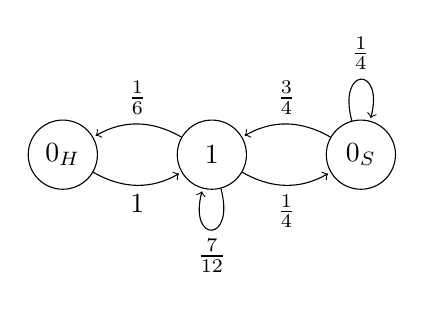
\begin{tikzpicture}
        \node[state]             (0) {$0_H$};
        \node[state, right=of 0] (2) {$1$};
        \node[state, right=of 2] (1) {$0_S$};

        \draw[every loop]
            (0) edge[bend right, auto=right]  node {1} (2)
            (2) edge[bend right, auto=right]  node {$\frac{1}{6}$} (0)
            (1) edge[loop above] node {$\frac{1}{4}$} (1)
            (2) edge[bend right, auto=right] node {$\frac{1}{4}$} (1)
            (1) edge[bend right, auto=right] node {$\frac{3}{4}$} (2)
            (2) edge[loop below] node {$\frac{7}{12}$} (2)
            ;
\end{tikzpicture}

\subsubsection*{ b) }

ergodic?
\begin{itemize}
\item  finite state space
\item  irreducible because single communicating class
\item  periodicity is same for all states in same class
\end{itemize}
$\rightarrow$ yes

\subsubsection*{ c) }

fraction working = $\pi_1$

\begin{align*}
\pi &= \pi \cdot P\\
\sum_{i=1}^3 \pi_i &= 1\\
P &= ((7/12,1/6,1/4),(1,0,0),(3/4,0,1/4))
\end{align*}

\begin{align*}
\pi _{1}\cdot \frac{1}{6}&=\pi _{{0_{H}}}\\
\pi _{1}&=6\cdot \pi _{{0_{H}}}\\
\pi _{1}\cdot \frac{1}{4}&=\frac{3}{4}\pi _{{0_{S}}}\\
\pi _{1}&=3\cdot \pi _{{0_{S}}}
\end{align*}

\begin{align*}
1&=\pi _{1}+\pi _{{0_{H}}}+\pi _{{0_{S}}}\\
1&=6\pi _{{0_{H}}}+\pi _{{0_{H}}}+2\pi _{{0_{H}}}
\end{align*}

\begin{align*}
\pi &=\left(\pi _{1},\pi _{{0_{H}}},\pi _{{0_{S}}}\right)=\left(\frac{6}{9},\frac{1}{9},\frac{2}{9}\right)
\end{align*}

The data center is up $\frac{2}{3}$ of the time

\subsubsection*{ d) }

mean time between backhoe failures = mean time between visits to $\pi _{0_H}$
\begin{align*}
E[T_{0_H}] = \frac{1}{\pi_{0_H}} = 9
\end{align*}

\subsubsection*{ 3. }

transition matrix P denotes the probabilities of following a link
 rank = r


$r_{{n+1}}=r_{n}\cdot P$\\
$r_{0} \rightarrow$  solvable if $P$ is ergodic, because then the limiting distribution exists\\
$n_{j}=$ nr of links on page i to j\\
$N_{i}=$  nr links on page i\\
$P_{{\left(i,j\right)}}=\frac{n_{j}}{N_{i}}$\\


\subsubsection*{ a) }
\begin{align*}
P&=\left(\left(0,\frac{1}{2},0,\frac{1}{2}\right),\left(0,0,\frac{1}{2},\frac{1}{2}\right),\left(1,0,0,0\right),\left(0,0,0,1\right)\right)
\end{align*}
\subsubsection*{ c) }
\begin{align*}
\pi&=\pi\cdot P\\
\pi_{1}+\pi_{2}+\pi_{3}+\pi_{4}&=1
\end{align*}
$\rightarrow$ $\pi=\left(0,0,0,1\right)$  is stationary distribution, if ergodic (see b) it is also limiting distribution.
That $\pi=\left(0,0,0,1\right)$ is the stationary distribution makes intuitive sense, since once we arrive on webpage 4
we can never leave it.

\subsubsection*{ b) }

ergodic?:\\
irreducible? $\rightarrow$ no: there are 2 classes $\{4\},\{1,2,3\}$\\
ergodicity is a sufficient but no necessary condition for the existence of a limiting distribution
eventually you will get stuck in state of page 4 so limiting distribution = stationary distribution

\subsubsection*{ d) }
with teleportation
\begin{align*}
P' &=\left(\left(0,\frac{1}{2},0,\frac{1}{2}\right),\left(0,0,\frac{1}{2},\frac{1}{2}\right),\left(1,0,0,0\right),\left(\frac{1}{3},\frac{1}{3},\frac{1}{3},0\right)\right)
\end{align*}
\subsubsection*{ e) }

now chain is irreducible, also aperiodic and the state space is finite $\rightarrow$ ergodic

\subsubsection*{ f) }
solve system of equations $\pi=\pi\cdot P'$ with  $\pi_{1}+\pi_{2}+\pi_{3}+\pi_{4}=1$\\
$\rightarrow$ $\pi=\frac{1}{102}\left(30,24,21,27\right)$

the limiting distribution defines final ranks for all pages

\subsection*{ 4. }

based on the edges of the CTMC we fill in the transition rate matrix Q that
defines the CTMC:
\begin{align*}
Q&=\left(\left(x,1,0\right),\left(2,y,2\right),\left(4,3,z\right)\right)\\
Q&=\left(\left(-1,1,0\right),\left(2,-4,2\right),\left(4,3,-7\right)\right)&& \text{-  rows have to sum to 0 -}
\end{align*}

We fill in the transition matrix $P$ for the corresponding DTMC, based on
$p_{{ij}}=\frac{q_{{ij}}}{-q_{{ii}}}$

\begin{align*}
P&=\left(\left(0,1,0\right),\left(\frac{1}{2},0,\frac{1}{2}\right),\left(\frac{4}{7},\frac{3}{7},0\right)\right)
\end{align*}

\subsection*{ 5. }

\subsubsection*{ a) }

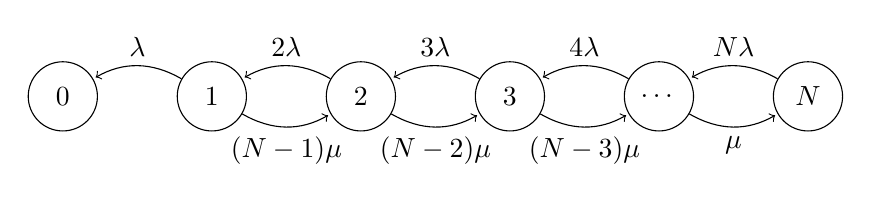
\begin{tikzpicture}
        \node[state]             (0) {0};
        \node[state, right=of 0] (1) {1};
        \node[state, right=of 1] (2) {2};
        \node[state, right=of 2] (3) {3};
        \node[state, right=of 3] (4) {\ldots};
        \node[state, right=of 4] (5) {$N$};

        \draw[every loop]
            (1) edge[bend right, auto=right] node {$\lambda$} (0)
            (1) edge[bend right, auto=right]  node {$(N-1)\mu$} (2)
            (2) edge[bend right, auto=right] node {$2 \lambda$} (1)
            (2) edge[bend right, auto=right]  node {$(N-2)\mu$} (3)
            (3) edge[bend right, auto=right] node {$3 \lambda$} (2)
            (3) edge[bend right, auto=right]  node {$(N-3)\mu$} (4)
            (4) edge[bend right, auto=right] node {$4 \lambda$} (3)
            (4) edge[bend right, auto=right]  node {$\mu$} (5)
            (5) edge[bend right, auto=right] node {$N\lambda$} (4)
            ;
\end{tikzpicture}


\begin{itemize}
\item  chain is a birth-death chain: the state transitions are of only two types: "births", which increase the state variable by one and "deaths", which decrease the state by one
\item  $\left(N-1\right)\mu $ because data of $\left(N-1\right)$ drives has to be copied
\item  $2\lambda $ because each of the drives can fail with rate $\lambda $ so we have to sum them
\item the chain is not ergodic since it is reducible to state 0
\end{itemize}

\subsubsection*{ b) }

limiting probability mass function $\rightarrow \left(1,0,0,\ldots ,0\right)$, in the long run you will
end up in state 0 and you will not be able to get out since there are no outgoing links.

\clearpage

\section{Birth Death Queues}

\subsection*{Preparatory Exercise}

definition exponential series:  $$e^z = \sum_{k=0}^{\infty} \frac{z^k}{k!}$$

\subsubsection*{1}

\begin{align*}
    z e^z &= z \sum_{k=0}^{\infty} \frac{z^k}{k!} \\
    &= z \sum_{k=1}^{\infty} \frac{z^{k-1}}{(k-1)!}\\
    &= \sum_{k=1}^{\infty} \frac{z^k}{(k-1)!} \\
    &= \sum_{k=1}^{\infty} k\frac{z^k}{k!} \\
    &= \sum_{k=0}^{\infty}{k\frac{z^k}{k!}} && \text{ - multiplication by zero adds nothing to sum - }
\end{align*}

\subsubsection*{2}

\begin{align*}
    (z + z^2) e^z &= z(z e^z+ e^z)\\
    &= z \left( \sum_{k=0}^{\infty}{k\frac{z^k}{k!}} + \sum_{k=0}^{\infty} \frac{z^k}{k!}\right) && \text{ - use previous identities - }\\
    &= z \left( \sum_{k=0}^{\infty}{k\frac{z^k}{k!}} + \sum_{k=1}^{\infty} \frac{z^{k-1}}{(k-1)!}\right) \\
    &= z \left( \sum_{k=1}^{\infty}{(k-1)\frac{z^{k-1}}{(k-1)!}} + \sum_{k=1}^{\infty} \frac{z^{k-1}}{(k-1)!}\right) \\
    &= z \sum_{k=1}^{\infty} k \frac{z^{k-1}}{(k-1)!} \\
    &= \sum_{k=0}^{\infty} k^2 \frac{z^k}{k!} \\
\end{align*}

\clearpage

\subsubsection*{3}

if $z = 1$ we have division by zero so we assume $z \neq 1$:

\begin{align*}
    1-z^{n+1} &= (1 - z) \sum_{k=0}^{n} z^k \\
    1-z^{n+1} &= (1 - z) \frac{1 - z^{n+1}}{1-z}  && \text{-http://mathworld.wolfram.com/GeometricSeries.html-}\\
    1-z^{n+1} &= 1-z^{n+1}
\end{align*}

\subsubsection*{4}

\begin{align*}
\sum_{k=0}^{n} k z^k &= z \sum_{k=0}^{n} k z^{k-1}\\
&= z \sum_{k=0}^{n} \frac{dz^k}{dz}\\
&= \frac{z}{dz} d \left( \sum_{k=0}^{n} z^k \right)\\
&= \frac{z}{dz} d \left(\frac{1 - z^{n+1}}{1-z}\right) && \text{-http://mathworld.wolfram.com/GeometricSeries.html-}\\
&= z \frac{1-(n+1)z^n + n z^{n+1}}{(1-z)^2} && \text{- derivative of fraction + simplify -}
\end{align*}

The infinite series have region of convergence $|z| \leq 1$ and limits:
$$ \lim_{n\to\infty} \sum_{k=0}^{n} z^k = \lim_{n\to\infty} \frac{1 - z^{n+1}}{1-z} = \frac{1}{1-z} $$
$$ \lim_{n\to\infty} \sum_{k=0}^{n} k z^k = \lim_{n\to\infty} \frac{z(1-(n+1)z^n + n z^{n+1})}{(1-z)^2} = \frac{z}{1-z^2} $$

\subsection*{ 1. }

\subsubsection*{ a) }

state space = $\mathbb{N}$, $S$ = system content.

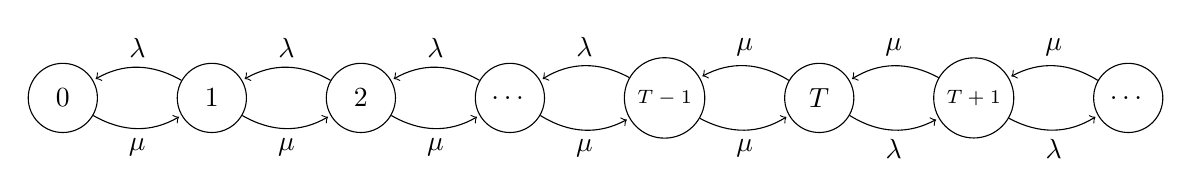
\begin{tikzpicture}
        \node[state]             (0) {0};
        \node[state, right=of 0] (1) {1};
        \node[state, right=of 1] (2) {2};
        \node[state, right=of 2] (3) {\ldots};
        \node[state, right=of 3] (4) {\scriptsize{$T-1$}};
        \node[state, right=of 4] (5) {$T$};
        \node[state, right=of 5] (6) {\scriptsize{$T+1$}};
        \node[state, right=of 6] (7) {\ldots};

        \draw[every loop]
            (0) edge[bend right, auto=right]  node {$\mu$} (1)
            (1) edge[bend right, auto=right] node {$\lambda$} (0)
            (1) edge[bend right, auto=right]  node {$\mu$} (2)
            (2) edge[bend right, auto=right] node {$\lambda$} (1)
            (2) edge[bend right, auto=right]  node {$\mu$} (3)
            (3) edge[bend right, auto=right] node {$\lambda$} (2)
            (3) edge[bend right, auto=right]  node {$\mu$} (4)
            (4) edge[bend right, auto=right] node {$\lambda$} (3)
            (4) edge[bend right, auto=right]  node {$\mu$} (5)
            (5) edge[bend right, auto=right] node {$\mu$} (4)
            (5) edge[bend right, auto=right]  node {$\lambda$} (6)
            (6) edge[bend right, auto=right] node {$\mu$} (5)
            (6) edge[bend right, auto=right]  node {$\lambda$} (7)
            (7) edge[bend right, auto=right] node {$\mu$} (6)
            ;
\end{tikzpicture}

\clearpage

\subsubsection*{ b) }

For which $\lambda ,\mu ,T$ is the Markov chain ergodic?
\begin{itemize}
\item chain is irreducible
\item is the chain positive recurrent ? $\rightarrow$ solve for stationary distribution:
\end{itemize}

detailed balance equations:
\begin{align*}
\left(1\right)\mu s\left(0\right)&=\lambda s\left(1\right)\\
\left(2\right)\mu s\left(n\right)&=\lambda s\left(n+1\right)&& \text{- n = 0,1, ..., T-2 -}\\
\left(3\right)\mu s\left(T-1\right)&=\mu s\left(T\right)\\
\left(4\right)\lambda s\left(n\right)&=\mu s\left(n+1\right)&& \text{- n = T+1, T+2... -}
\end{align*}

$\rho =\frac{\lambda }{\mu }$

\begin{align*}
\left(1\right)&\Rightarrow s\left(1\right)=\frac{\mu }{\lambda }s\left(0\right)=\frac{1}{\rho }s\left(0\right)\\
\left(2\right)&\Rightarrow s\left(n+1\right)=\frac{\mu }{\lambda }s\left(n\right)=\frac{\mu }{\lambda }\cdot \frac{\mu }{\lambda }\cdot s\left(n-1\right)\\
&=\ldots=\frac{1}{\rho ^{\left(n+1\right)}}\cdot s\left(0\right)&& \text{- n=0,1,...,T-2 -}\\
\left(3\right)&\Rightarrow s\left(T\right)=s\left(T-1\right)=\frac{1}{\rho ^{\left(T-1\right)}}\cdot s\left(0\right)\\
\left(4\right)&\Rightarrow s\left(n\right)=\frac{\lambda }{\mu }s\left(n-1\right)=\rho \cdot s\left(n-1\right) && \text{- n = T+1, T+2... -}\\
&=\ldots=\rho ^{n-T}s\left(T\right)=\rho ^{\left(n+1-2T\right)}s\left(0\right)
\end{align*}
So:

\begin{align*}
s\left(n\right)&=\frac{1}{\rho ^{n}}s\left(0\right)&& \text{- n=0,1,...,T-2 -}\\
s\left(T\right)&=s\left(T-1\right)=\frac{1}{\rho ^{\left(T-1\right)}}s\left(0\right)\\
s\left(n\right)&=\rho ^{\left(n-2T+1\right)}s\left(0\right)&& \text{-  $n=T+1,\ldots$ -}\\
1&=\sum_{{n=0}}^{\infty}s\left(n\right)=s\left(0\right)\cdot \left(\sum _{{n=0}}^{{T-1}}\frac{1}{\rho ^{n}}+\frac{1}{\rho ^{{T-1}}}+\sum _{{n=T+1}}^{\infty}\rho ^{{n-2T+1}}\right)\\
&=s\left(0\right)\cdot \left(\frac{1-\left(\rho ^{{-1}}\right)^{T}}{1-\rho ^{{-1}}}+\frac{1}{\rho ^{{T-1}}}+\sum _{{n=T+1}}^{\infty}\rho ^{{n-2T+1}}\right) && \text{- $\sum_{k=0}^{n} z^k = \frac{1 - z^{n+1}}{1-z}$ -}\\
&=s\left(0\right)\cdot \left(\frac{1-\left(\rho ^{{-1}}\right)^{T}}{1-\rho ^{{-1}}}+\sum _{{n=T}}^{\infty}\rho ^{{n-2T+1}}\right) && \text{- include $\frac{1}{\rho ^{{T-1}}}$ in summation -}\\
&= s\left(0\right)\cdot \frac{1-\left(\rho ^{-1}\right)^T}{1-\rho ^{-1}} + \rho ^{{-T+1}}\cdot \frac{1}{1-\rho } && \text{- $\sum _{{n=T}}^{\infty} \rho ^{n}=\frac{\rho ^{T}}{1-\rho }$ -}
\end{align*}

$\Rightarrow s\left(0\right)=\frac{\rho ^{{T-1}}\left(1-\rho \right)}{1-\rho ^{T}}$

Markov chain is ergodic when:\\
\begin{itemize}
\item To have s(0) positive, you need: $2-\rho ^{T}> 0 \Leftrightarrow \rho ^{T}< 2$
\item T is finite
\item $0< \rho < 1$
\end{itemize}

\subsubsection*{ c) }

\begin{align*}
E\left[N\right]&=\sum _{{n=0}}^{\infty}n\cdot s\left(n\right)\\
&=\ldots\\
&=\frac{\left(1-\rho \right)\left(2T-1\right)+\rho ^{T}}{\left(1-\rho \right)\left(2\cdot \rho ^{T}\right)}\\
&=\frac{2T-1}{2\rho ^{T}}+\frac{\rho ^{T}}{\left(1-\rho \right)\left(2-\rho ^{T}\right)}
\end{align*}

\subsection*{ 2. }

\subsubsection*{ a) }

\begin{tikzpicture}
        \node[state]             (0) {0};
        \node[state, right=of 0] (1) {$1_1$};
        \node[state, below=of 3] (2) {$1_2$};
        \node[state, right=of 1] (3) {2};
        \node[state, right=of 3] (4) {3};
        \node[state, right=of 4] (5) {4};
        \node[state, right=of 5] (6) {5};
        \node[state, right=of 6] (7) {\ldots};

        \draw[every loop]
            (0) edge[bend right, auto=left]  node {$\lambda$} (1)
            (1) edge[bend right, auto=right] node {$\mu_1$} (0)
            (2) edge[bend left, auto=left]  node {$\mu_2$} (0)
            (3) edge[bend right=50, auto=right]  node {$\mu_1$} (2)
            (2) edge[bend left, auto=right] node {$\lambda$} (3)
            (3) edge[bend right, auto=right]  node {$\mu_2$} (1)
            (1) edge[bend right, auto=right] node {$\lambda$} (3)
            (3) edge[bend right, auto=left]  node {$\lambda$} (4)
            (4) edge[bend right, auto=right] node {$\mu_1 + \mu_2$} (3)
            (4) edge[bend right, auto=right]  node {$\lambda$} (5)
            (5) edge[bend right, auto=right] node {$\mu_1 + \mu_2$} (4)
            (5) edge[bend right, auto=right]  node {$\lambda$} (6)
            (6) edge[bend right, auto=right] node {$\mu_1 + \mu_2$} (5)
            (6) edge[bend right, auto=right]  node {$\lambda$} (7)
            (7) edge[bend right, auto=right] node {$\mu_1 + \mu_2$} (6)
            ;
\end{tikzpicture}

\subsubsection*{ b) }

irriducible $\rightarrow$ clear from state diagram\\
\textbf{to prove}: stationary probability mass function\\
local balance equations $\rightarrow$ combine states instead of writing down local ones state by state $\rightarrow$ is equivalent

\begin{align*}
\left(1\right)\lambda s\left(0\right)&=\mu _{1}s\left(1,1\right)+\mu _{2}s\left(1,2\right)\\
\left(2\right)\lambda \cdot s\left(1,1\right)&=\mu _{2}s\left(2\right)+\mu _{1}\cdot s\left(1,2\right)\\
\left(3\right)\left(\lambda +\mu _{2}\right)s\left(1,2\right)&=\mu _{1}s\left(2\right)\\
\left(4\right)\lambda s\left(n\right)&=\left(\mu _{1}+\mu _{2}\right)s\left(n+1\right) \text{ - n=2,3,\ldots - }
\end{align*}

$\rho =\frac{\lambda }{\mu _{1}+\mu _{2}}$

After some calculations:

\begin{align*}
s\left(1,1\right)&=\frac{\lambda \left(1+\rho \right)}{\mu _{1}\left(1+2\rho \right)}s\left(0\right)\\
s\left(1,2\right)&=\frac{\lambda \cdot \rho }{\mu _{2}\cdot \left(1+2\rho \right)}s\left(0\right)\\
s\left(n\right)&=\frac{\left(\lambda +\mu _{2}\right)\cdot \lambda }{\mu _{1}\cdot \mu _{2}}\cdot \frac{\rho ^{{n+1}}}{1+2\rho }s\left(0\right)\text{ - $n=2,3\ldots$ - }
\end{align*}

\begin{align*}
s\left(1,1\right)+s\left(1,2\right)&=s\left(0\right)\cdot \frac{\lambda \left(\lambda +\mu _{2}\right)}{\mu _{1}\mu _{2}\left(1+2\rho \right)}
\end{align*}
\begin{align*}
1&=\sum _{{n=0}}^{\infty}s\left(n\right)=s\left(0\right)\left(\ldots\right)
\end{align*}

\begin{align*}
s\left(0\right)=\left(1+\left(\lambda \frac{\lambda +\mu _{2}}{\mu _{1}\mu _{2}\left(1+2\rho \right)\left(1-\rho \right)}\right)\right)^{{-1}}
\end{align*}

if $0< \rho < 1$ the markov chain is ergodic

\subsubsection*{ c) }
\begin{align*}
E\left[N\right]&=\sum _{{n=0}}^{\infty }n\cdot s\left(n\right)\\
&=\ldots \\
&=\frac{1}{\frac{\mu _{1}\mu _{2}\left(1+2\rho \right)}{\lambda \left(\lambda +\mu _{2}\right)}+\frac{1}{1-\rho }}\\
&=\frac{1}{0+\frac{1}{1-\rho }}\cdot \frac{1}{\left(1-\rho \right)^{2}}\\
&=\frac{1-\rho }{\left(1-\rho \right)^{2}}\\
&=\frac{1}{1-\rho }
\end{align*}
\subsubsection*{ d) }

$\lambda < \mu _{1}+\mu _{2}$

if $\mu _{2}< < \mu _{1}$, then $\rho \approx \frac{\lambda }{\mu _{1}}$, fill these params in in c) $\Rightarrow E\left[N\right]\approx \frac{1}{1-\rho }$\\
For a M/M/1 with params $\left(\lambda ,\mu _{1}\right)$ -see syllabus- than we know $E\left[N\right]=\frac{\rho }{1-\rho }$ with $\rho =\frac{\lambda }{\mu _{1}}< 1$,\\
this is smaller than before hence it is faster to use 1 server.

Conclusion : if server 2 is much slower than server 1 you are better off without server 2\\
better to let a customer wait a bit longer and then serve them quicker\\
the mean waiting time will increase a bit but the mean sojourn time will decrease much more\\

\subsection*{ 3. }

\subsubsection*{ a) }

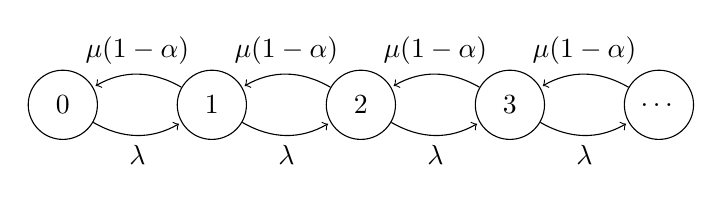
\begin{tikzpicture}
        \node[state]             (0) {0};
        \node[state, right=of 0] (1) {1};
        \node[state, right=of 1] (2) {2};
        \node[state, right=of 2] (3) {3};
        \node[state, right=of 3] (4) {\ldots};

        \draw[every loop]
            (0) edge[bend right, auto=right]  node {$\lambda$} (1)
            (1) edge[bend right, auto=right] node {$\mu(1-\alpha)$} (0)
            (1) edge[bend right, auto=right]  node {$\lambda$} (2)
            (2) edge[bend right, auto=right]  node {$\mu(1-\alpha)$} (1)
            (2) edge[bend right, auto=right] node {$\lambda$} (3)
            (3) edge[bend right, auto=right]  node {$\mu(1-\alpha)$} (2)
            (3) edge[bend right, auto=right] node {$\lambda$} (4)
            (4) edge[bend right, auto=right]  node {$\mu(1-\alpha)$} (3)
            ;
\end{tikzpicture}

The feedback can be simplified by setting the service rate to $\mu(1-\alpha)$,\\
which results in a normal M/M/1 queue

\subsubsection*{ b) }

$s\left(0\right)$ ?

\begin{align*}
\lambda s\left(n-1\right)&=\mu \left(1-\alpha \right)s\left(n\right) && \text{- $n=1,2,\ldots$ -}\\
s\left(n\right)&=\left(\frac{\lambda }{\mu \left(1-\alpha \right)}\right)^{n}s\left(0\right)\\
s(n) &=\rho ^{n}s\left(0\right)&& \text{-  with $\rho =\frac{\lambda }{\mu \left(1-\alpha \right)}$ -}
\end{align*}

\begin{align*}
1&=\sum _{{n=0}}^{\infty}s(n)\\
&=s\left(0\right)\sum _{{n=0}}^{\infty}\rho ^{n}\\
&=s\left(0\right)\frac{1}{1-\rho }&& \text{-  if $0< \rho < 1$ then ergodic -}\\
s(0) &= 1 - \rho
\end{align*}

\subsubsection*{ c) }

\begin{align*}
E\left[N\right]&=\sum _{{n=0}}^{\infty}n\cdot s\left(n\right)\\
&=\sum _{{n=1}}^{\infty}n\cdot \rho ^{n}\cdot \left(1-\rho \right) && \text{ - leave out multiplication by zero - }\\
&=\frac{\rho }{1-\rho }
\end{align*}

\subsection*{ 4. }

\subsubsection*{ a) }

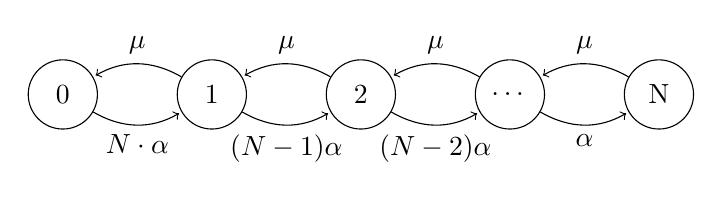
\begin{tikzpicture}
        \node[state]             (0) {0};
        \node[state, right=of 0] (1) {1};
        \node[state, right=of 1] (2) {2};
        \node[state, right=of 2] (3) {\ldots};
        \node[state, right=of 3] (4) {N};

        \draw[every loop]
            (0) edge[bend right, auto=right]  node {$N \cdot \alpha$} (1)
            (1) edge[bend right, auto=right] node {$\mu$} (0)
            (1) edge[bend right, auto=right]  node {$(N-1)\alpha$} (2)
            (2) edge[bend right, auto=right]  node {$\mu$} (1)
            (2) edge[bend right, auto=right] node {$(N-2)\alpha$} (3)
            (3) edge[bend right, auto=right]  node {$\mu$} (2)
            (3) edge[bend right, auto=right] node {$\alpha$} (4)
            (4) edge[bend right, auto=right]  node {$\mu$} (3)
            ;
\end{tikzpicture}

\subsubsection*{ b) }

$s\left(n\right)=Prob\left(N-n\right)$

detailed balance equations:

\begin{align*}
\left(1\right)N\cdot \alpha \cdot s\left(0\right)&=\mu s\left(1\right)\\
\left(2\right)\left(N-1\right)\cdot \alpha \cdot s\left(1\right)&=\mu s\left(2\right)\\
\left(n\right)\left(N-n+1\right)\cdot \alpha \cdot s\left(n-1\right)&=\mu \cdot s\left(n\right)&& \text{- $n=1,2,\ldots,N$ -}
\end{align*}

$s\left(n\right)=c_{n}\cdot s\left(0\right)$

\begin{align*}
s\left(n\right)&=\frac{\left(N-\left(n-1\right)\right)}{\mu }\cdot \alpha \cdot s\left(n-1\right)\\
&=\frac{\left(N-\left(n-1\right)\right)}{\mu }\cdot \frac{\left(N-\left(n-2\right)\right)}{\mu }\cdot \alpha \cdot \left(s\left(n-2\right)\right)\\
&=\frac{\left(N-\left(n-1\right)\right)\cdot \alpha }{\mu }\cdot \ldots\cdot \frac{N\alpha }{\mu }\cdot s\left(0\right)\\
&=\frac{N!}{\left(N-n\right)!}\cdot \left(\frac{\alpha }{\mu }\right)^{n}\cdot s\left(o\right)&& \text{-  $\forall n$ in $\mathbb{N}, \prod _{{i=1}}^{n}N-(n-i) = \frac{N!}{\left(N-n\right)!}$ -}
\end{align*}

\begin{align*}
1&=\sum _{{n=0}}^{N}s\left(n\right)\\
&=\left(\sum _{{n=0}}^{N}\frac{N!}{\left(N-n\right)!}\cdot \left(\frac{\alpha }{\mu }\right)^{n}\right)s\left(0\right)
\end{align*}

$\rightarrow$ $s\left(0\right)=\left(\sum _{{n=0}}^{N}\frac{N!}{\left(N-n\right)!}\cdot \left(\frac{\alpha }{\mu }\right)^{n}\right)^{{-1}}$

\subsubsection*{ c) }

$\left(Pr\left(\mu =n\right)=Pr\left(N-S=n\right)\right)=s\left(N-n\right)\forall n$ in $\{0,1,\ldots,N\}$

$Pr\left(\mu =n\right)$ $\rightarrow$ prob n users are analyzing completed job ( preparing new job )

$Pr\left(N-S=n\right)$ $\rightarrow$ prob N-n jobs are in the system

\subsection*{ 5. }

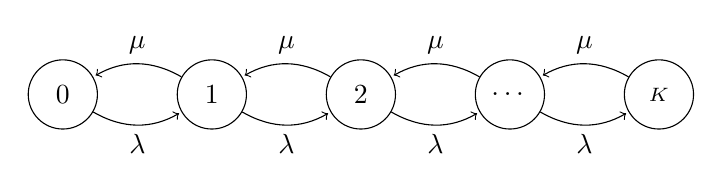
\begin{tikzpicture}
        \node[state]             (0) {0};
        \node[state, right=of 0] (1) {1};
        \node[state, right=of 1] (2) {2};
        \node[state, right=of 2] (3) {\ldots};
        \node[state, right=of 3] (4) {\scriptsize{$K$}};

        \draw[every loop]
            (0) edge[bend right, auto=right]  node {$\lambda$} (1)
            (1) edge[bend right, auto=right] node {$\mu$} (0)
            (1) edge[bend right, auto=right]  node {$\lambda$} (2)
            (2) edge[bend right, auto=right] node {$\mu$} (1)
            (2) edge[bend right, auto=right]  node {$\lambda$} (3)
            (3) edge[bend right, auto=right] node {$\mu$} (2)
            (3) edge[bend right, auto=right]  node {$\lambda$} (4)
            (4) edge[bend right, auto=right] node {$\mu$} (3)
            ;
\end{tikzpicture}

\begin{align*}
\lambda s\left(n-1\right)&=\mu s\left(n\right)&& \text{-  $n=1,2\ldots $ -}\\
s\left(1\right)&=\rho s\left(0\right) && \text{-  $\rho =\frac{\lambda }{\mu }$ -}\\
s\left(2\right)&=\rho ^{2}s\left(0\right)\\
s\left(K\right)&=\rho ^{K}s\left(0\right)
\end{align*}

\begin{align*}
1&=\sum _{{n=0}}^{K}s\left(n\right)\\
&= s(0) \cdot \sum_{{n=0}}^{K} \rho^n\\
&= s(0) \frac{1-\rho ^{{K+1}}}{1-\rho }
\end{align*}

\begin{align*}
s(K)&= \rho ^{K}\frac{1-\rho }{1-\rho ^{{K+1}}}
\end{align*}

\subsubsection*{ a) }

Assume $\rho=0.4$.
Doubling the service rate (using $\mu' = 2 \mu$) results in a halving of the load:
\[
\rho' = \frac{\lambda}{2 \mu} = \frac{\rho}{2}.
\]
The requested loss probabilities are summarized in the following table:
\begin{table}[H]
\centering
\begin{tabular}{ccc}
$\rho$  & $K$   & $p_{\text{loss}}$ \\ \hline
0.4     & 5     & $6 \cdot 10^{-3}$ \\
0.2     & 5     & $3 \cdot 10^{-4}$ \\
0.4     & 10    & $6 \cdot 10^{-5}$
\end{tabular}
\end{table}
Doubling the system capacity has a greater (positive) effect on the loss probability.

\subsubsection*{ b) }

Assume $\rho=0.8$.
The requested loss probabilities are summarised in the following table:
\begin{table}[H]
\centering
\begin{tabular}{ccc}
$\rho$  & $K$   & $p_{\text{loss}}$ \\ \hline
0.8     & 5     & $9 \cdot 10^{-2}$ \\
0.4     & 5     & $6 \cdot 10^{-3}$ \\
0.8     & 10    & $2 \cdot 10^{-2}$
\end{tabular}
\end{table}
Doubling the service rate has a greater (positive) effect on the loss probability.

\subsubsection*{ c) }
The intuitive solution would be to increase the system capacity.
If the load is high, then the system will be at full capacity for a large proportion of the time, even if the system has a high capacity.

\subsection*{ 6. }

\subsubsection*{ a) }

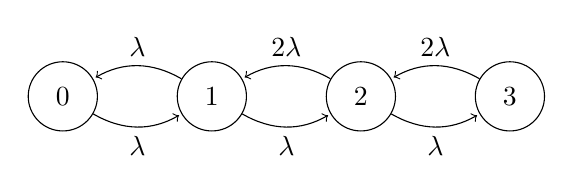
\begin{tikzpicture}
        \node[state]             (0) {0};
        \node[state, right=of 0] (1) {1};
        \node[state, right=of 1] (2) {2};
        \node[state, right=of 2] (3) {3};

        \draw[every loop]
            (0) edge[bend right, auto=right]  node {$\lambda$} (1)
            (1) edge[bend right, auto=right] node {$\lambda$} (0)
            (1) edge[bend right, auto=right]  node {$\lambda$} (2)
            (2) edge[bend right, auto=right]  node {$2\lambda$} (1)
            (2) edge[bend right, auto=right] node {$\lambda$} (3)
            (3) edge[bend right, auto=right]  node {$2\lambda$} (2)
            ;
\end{tikzpicture}

$2 \lambda$ because once there are two tasks two servers can work on it.

\subsubsection*{ b) }

two costumers $\rightarrow s=2$\\
$T_a \sim Exp(|\lambda), T_d \sim Exp( | 2 \cdot \lambda)$

\begin{align*}
Pr\left(\text{arrival before departure}\right)&=Pr\left[T_{a}< T_{d}\right]\\
&=\int _{0}^{\infty }Pr\left(t< T_{d}\right)f_{a}\left(t\right)dt\\
&=\int _{0}^{\infty }(1-F_{T_d}(t))f_{a}\left(t\right)dt\\
&=\int _{0}^{\infty }e^{{-2\lambda t}}\lambda e^{{-\lambda t}}dt&& \text{-  see table 1, A1.11 -}\\
&=\int _{0}^{\infty }\lambda \cdot e^{{-3\lambda t}}dt\\
&=\lambda \cdot \int _{0}^{\infty }e^{{-3\lambda t}}dt\\
&=\lambda \cdot \left[\frac{e^{{-3\lambda t}}}{-3\lambda }\right]_{0}^{\infty}\\
&=\lambda \cdot\left [0-\frac{1}{-3 \cdot \lambda}\right]\\
&=\frac{1}{3}
\end{align*}

\subsubsection*{ c) }

$s\left(n\right)=\lim_{{t\rightarrow \infty}}Pr\left[x_{t}=n\right]$  $n=0,1,2,3,\ldots$

detailed balance equations:

\begin{align*}
\left(1\right)\lambda s\left(0\right)&=\lambda s\left(1\right)\Rightarrow s\left(1\right)=s\left(0\right)\\
\left(2\right)\lambda s\left(1\right)&=2\lambda s\left(2\right)\Rightarrow s\left(2\right)=\frac{1}{2}s\left(1\right)=\frac{1}{2}s\left(0\right)\\
\left(3\right)\lambda s\left(2\right)&=2\lambda s\left(3\right)\Rightarrow s\left(3\right)=\frac{1}{2}s\left(2\right)=\frac{1}{2}\cdot \frac{1}{2}\cdot s\left(0\right)
\end{align*}

$1=s\left(0\right)\left(1+1+\frac{1}{2}+\frac{1}{4}\right)=\frac{11}{4}$

\begin{align*}
s\left(0\right)&=\frac{4}{11}\\
s\left(1\right)&=\frac{4}{11}\\
s\left(2\right)&=\frac{2}{11}\\
s\left(3\right)&=\frac{1}{11}
\end{align*}


\subsubsection*{ d) }

$E\left[S\right]=\sum _{{n=0}}^{3}n\cdot s\left(n\right)=1$

$0\cdot \frac{4}{11}+1\cdot \frac{4}{11}+2\cdot \frac{2}{11}+3\cdot \frac{1}{11}$

\subsubsection*{ e) }

probability of loss = prob arrival in state 3, there is no state 4, hence the customer will be lost:\\
$p_{loss}=s\left(3\right)=\frac{1}{11}$ (PASTA)

\subsubsection*{ f) }

\begin{align*}
\mu _{1}&=\lambda \\
\mu _{2}&=\mu _{3}=2\cdot \lambda 
\end{align*}

\begin{align*}
\mu _{{eff}}&=\sum _{{n=1}}^{3}s\left(n\right)\mu _{n}\\
&=\frac{10}{11}\lambda && \text{-  nr of leaving customers per second -}
\end{align*}

$\rightarrow$ $\frac{10}{11}\lambda \left[s^{{-1}}\right]=\left(1-p_{loss}\right)\cdot \lambda =\frac{10}{11}\lambda $

$\rightarrow$ $\mu _{eff}=\left(1-p_{loss}\right)\cdot \lambda =\lambda _{eff}$\\
this should always be the case: states system is in equilibrium:
at every time instant\\
nr incoming customers = nr outgoing customers

\subsubsection*{ g) }

An effective arrival occurs when a new customer arrives and the system is not full.
    The distribution of the number of customers in the system at an effective arrival is
    \[
        Pr[S_{A,eff} = n] = Pr[S_A = n | S_A < 3]
    \]
    where $S_{A,\text{eff}}$ is the system content at an effective arrival and $S_A$ is the system content at an arrival.
    From the PASTA (Poisson Arrivals See Time Averages) property and the ergodicity of the CTMC, it follows that $S_A = S$.
    Therefore
    \begin{align*}
        Pr[S_{A,eff} = n]
        &= Pr[S = n | S < 3]\\
        &= \frac{Pr[S = n, S < 3]}{Pr[S < 3]}\\
        &= \frac{Pr[S = n, S < 3]}{\frac{10}{11}}\\
    \end{align*}
    $s(n) = Pr[S = n, S < 3] \rightarrow s(n)$ is already calculated with $S < 3$\\
    which yields $Pr[S_{A,eff} = 0] = \dfrac{\dfrac{4}{11}}{\dfrac{10}{11}} = \frac{2}{5}$, $Pr[S_{A,eff} = 1] = \frac{2}{5}$ and $Pr[S_{A,eff] = 2} = \frac{1}{5}$.


\subsubsection*{ h) }

The rate of a Poisson process is constant, and knowing when the previous Poisson event has happened
is irrelevant for the occurrence of the next Poisson event.
In this case, this means that the effective arrival rate $\lambda_{eff}$ should be equal
to the effective arrival rate $\lambda_{a}$ right after an arrival.
By definition,
    \[
        \lambda_{eff}
        = ( 1 - s(3) ) \lambda = ( 1 - p_{\text{loss}}) \lambda = \frac{10}{11} \lambda.
    \]
    The effective arrival rate $\lambda_a$ right after an arrival can be calculated similarly, but now the loss probability is different.
    The probability mass function of the system content $S_a$ right after an effective arrival is computed from the relation
    \[
        Pr[S_a = n] = Pr[S = n | S > 0] = \frac{s(n)}{1 - s(0)},
    \]
    if $n$ is equal to 1, 2 or 3.
    We find
    \[
        \lambda_a = \frac{s(1) + s(2)}{1 - s(0)} \lambda = \frac{6}{7} \lambda.
    \]
    As $\lambda_{eff} \neq \lambda_a$, the effective arrival process is not a Poisson process.



\section{waiting times and delay}

\subsection*{ 1. }

\subsubsection*{ a) }

\textbf{used formulas}

stationary distribution M/M/1: $s_{{\rho \left(n\right)}}=\left(1-\rho \right)\cdot \rho ^{n}$

\textbf{solution}

\begin{align*}
Pr\left[S_{{\rho }}\le n\right] \text{ - $n \in \mathbb{N}$ - }
=\sum _{{i=0}}^{n}Pr\left(S_{{\rho }}=i\right)
\end{align*}

stationary distribution for M/M/1:
$s_{{\rho \left(n\right)}}=\left(1-\rho \right)\cdot \rho ^{n}$

\begin{align*}
Pr\left(S_{\rho }\le n\right)&=\sum _{{k=0}}^{n}Pr\left(S_{\rho }=k\right)\\
&=\sum _{{k=0}}^{n} s_{\rho }(k)\\
&=\left(1-\rho \right)\sum _{{k=0}}^{n}\rho ^{k}\\
&=\left(1-\rho \right)\frac{1-\rho ^{\left(n+1\right)}}{1-\rho }\\
&=1-\rho ^{{n+1}}
\end{align*}

$\forall x \in \mathbb{R}:Pr\left(S_{\rho }\le x\right)=1-\rho ^{{\lfloor x\rfloor+1}}$

\subsubsection*{ b) }

\textbf{used formulas}

Hopital:
\begin{align*}
\text{if } \lim _{{x\rightarrow a}}f\left(x\right)&=\lim _{{x\rightarrow a}}g\left(x\right)=0 \text{ or } \pm\infty \\
\lim _{{x\rightarrow a}}\frac{f\left(x\right)}{g\left(x\right)}&=\lim _{{x\rightarrow a}}\frac{f' \left(x\right)}{g' \left(x\right)}
\end{align*}

\textbf{solution}

\begin{align*}
Pr\left[\left(1-\rho \right)S_{\rho }\le x\right]&=Pr\left[S_{\rho }\le \frac{x}{1-\rho }\right]\\
&=1-\rho ^{{\frac{x}{\lfloor1-\rho \rfloor}+1}} && \text{ - fill in from a) -}
\end{align*}
\begin{align*}
1-\rho ^{{\frac{x}{1-\rho }}}\le 1-\rho ^{{\frac{x}{\lfloor1-\rho \rfloor}+1}}\le 1-\rho ^{{\frac{x}{1-\rho }+1}}
\end{align*}
solve limit from both sides, side one:
\begin{align*}
\lim_{{\rho \rightarrow 1}}\rho ^{{\frac{x}{1-\rho }}}&=\lim_{{\rho \rightarrow 1}}\exp\left(\ln\left(\rho^{\frac{x}{1-\rho }} \right)\right) &&
\text{$f(x)=e^{ln(f(x))}$}\\
&= \lim_{{\rho \rightarrow 1}}\exp\left(\frac{x}{1-\rho }\ln\left(\rho \right)\right) && \text{ - log power rule - }\\
&= \exp\left(\lim_{{\rho \rightarrow 1}}\frac{x}{1-\rho }\ln\left(\rho \right)\right) && \text{ - pass limit through exponential - }\\
&= \exp\left(x \cdot \lim_{{\rho \rightarrow 1}}\frac{ln(\rho)}{1-\rho }\right) && \text{ - factor out constant x - }\\
&=\exp\left(x \cdot \lim_{{\rho \rightarrow 1}}\left(\frac{\frac{1}{\rho }}{-1}\right)\right) && \text{ - hopital - }\\
&=\exp\left(x \cdot \lim_{{\rho \rightarrow 1}}\left(\frac{\rho }{-1}\right)\right)\\
&=\exp\left(-x\right)
\end{align*}
side two:
\begin{align*}
&=\lim_{{\rho \rightarrow 1}} \rho ^{{\frac{x}{1-\rho }+1}}\\
&=\exp\left(-x\right)
\end{align*}

combine boths sides $\rightarrow$ $\lim_{{\rho \rightarrow 1}}\left(1-\rho ^{{\frac{x}{\lfloor1-\rho \rfloor}+1}}\right)=1-\exp\left(-x\right)$

$\rightarrow$ When $\rho $ goes to 1, this distribution is converging to an exponential
distribution with $\lambda = 1$

\subsection*{ 2. }

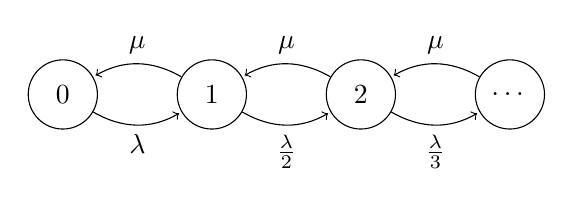
\begin{tikzpicture}
        \node[state]             (0) {0};
        \node[state, right=of 0] (1) {1};
        \node[state, right=of 1] (2) {2};
        \node[state, right=of 2] (3) {\ldots};

        \draw[every loop]
            (0) edge[bend right, auto=right]  node {$\lambda$} (1)
            (1) edge[bend right, auto=right] node {$\mu$} (0)
            (1) edge[bend right, auto=right]  node {$\frac{\lambda}{2}$} (2)
            (2) edge[bend right, auto=right]  node {$\mu$} (1)
            (2) edge[bend right, auto=right] node {$\frac{\lambda}{3}$} (3)
            (3) edge[bend right, auto=right]  node {$\mu$} (2)
            ;
\end{tikzpicture}

\subsubsection*{ a) }

$\lambda _{n}=$arrival rate when n customers in the system\\
$\mu _{n}=$service rate when n customers in the system

balance equations:

$s\left(n\right)\cdot \lambda _{n}=s\left(n+1\right)\mu _{{n+1}}$

Normalization condition:

$\sum _{{n=0}}^{\infty }s\left(n\right)=1$

\begin{align*}
\lambda _{n}&=\frac{\lambda }{n+1} && \text{ - $\forall n\in \mathbb{N}$ - }\\
\mu _{n }&=\mu && \text{ - $\forall n\in \mathbb{N}$ - }
\end{align*}

\textbf{Balance equations:}
\begin{align*}
s\left(n+1\right)&=s\left(n\right)\cdot \frac{\lambda }{\left(n+1\right)\mu }\\
&=s\left(n-1\right)\cdot \frac{\lambda }{n\mu }\cdot \frac{\lambda }{\left(n+1\right)\mu }\\
&=s\left(0\right)\cdot \left(\frac{\lambda }{\mu }\right)^{{n+1}}\cdot \frac{1}{\left(n+1\right)!}
\end{align*}

\begin{align*}
\sum _{{n=0}}^{\infty }s\left(n\right)&=1\\
s\left(0\right)\cdot \sum _{{n=0}}^{\infty }\left(\frac{\lambda }{\mu }\right)^{n}\cdot \frac{1}{n!} &= 1\\
s\left(0\right)&=\exp \left(-\frac{\lambda }{\mu }\right) && \text{- def exp series:  $e^z = \sum_{k=0}^{\infty} \frac{z^k}{k!}$ - }
\end{align*}
\begin{align*}
s\left(n\right)&=e^{{-\frac{\lambda }{\mu }}}\left(\frac{\lambda }{\mu }\right)^{n}\frac{1}{n!} && \text{ - $n\in \mathbb{N}$ - }
\end{align*}

\subsubsection*{ b) }

\textbf{used formulas}

definition laplace transform = 
\begin{align*}
\mathcal{L}\{f(t)\} &= \int_0^{\infty} e^{- s t} f(t) dt && \text{- with s a complex var - }\\
&= E[e^{- s W}]
\end{align*}

\begin{align*}
\hat{s}(n): \text{distr after departure}\\
\widetilde{s}(n): \text{distr before departure}\\
\widetilde{s}(n+1) = \hat{s}(n)\\
\end{align*}

\textbf{solution}

We use a different approach then usual, because $\lambda$ is not fixed,\\
hence PASTA does not apply and so $S_A = S$ does not apply.\\
We use a more broadly applicable approach here\\

\begin{align*}
D^{\ast }\left(s\right) &= \text{laplace transform of the delay of a customer}\\
&=E\left[e^{{-s\cdot W}}\right]\\
&=\sum _{n}E\left[e^{{-sW}}|S^{A}=n\right]\cdot \hat{s}\left(n\right)
\end{align*}
\begin{align*}
\hat{s}\left(n\right)&=\widetilde{s}\left(n+1\right) \text{ - distr seen by someone just before departure - }\\
\widetilde{s}\left(n\right)&=\frac{s\left(n\right)}{1-s\left(0\right)} \text{ You can't have a departure when the system content is 0.}
\end{align*}

\begin{align*}
\hat{s}\left(n\right)&=\widetilde{s}\left(n+1\right)\\
&=\frac{s\left(n+1\right)}{1-s\left(0\right)} && \text{ - see earlier result - }\\
&=\frac{e^{{-\frac{\lambda }{\mu }}}\left(\frac{\lambda }{\mu }\right)^{{n+1}}\frac{1}{\left(n+1\right)!}}{1-e^{{-\frac{\lambda }{\mu }}}} && \text{ - fill in from a) -}
\end{align*}

$E\left[e^{{-sW}}|S^{A}=n\right]=\left(\frac{\mu }{\mu +s}\right)^{{n+1}}$ see formula p 3.11

\begin{align*}
D^{\ast }\left(s\right) &= \sum _{n}E\left[e^{{-sW}}|S^{A}=n\right]\cdot \hat{s}\left(n\right)\\
&=\sum _{{n=0}}^{\infty }\left(\frac{\mu }{\mu +s}\right)^{{n+1}}\cdot \frac{e^{{-\frac{\lambda }{\mu }}}\left(\frac{\lambda }{\mu }\right)^{{n+1}}\frac{1}{\left(n+1\right)!}}{1-e^{{-\frac{\lambda }{\mu }}}}\\
&=\frac{e^{{-\frac{\lambda }{\mu }}}}{1-e^{{-\frac{\lambda }{\mu }}}}\cdot \sum _{{n=0}}^{\infty }\left(\frac{\mu }{\mu +s}\right)^{{n+1}}\left(\frac{\lambda }{\mu }\right)^{{n+1}}\frac{1}{\left(n+1\right)!}\\
&=\frac{e^{{-\frac{\lambda }{\mu }}}}{1-e^{{-\frac{\lambda }{\mu }}}}\cdot \sum _{{n=1}}^{\infty }\left(\frac{\lambda }{\mu +s}\right)^{{n}}\frac{1}{n!}\\
&=\frac{e^{{-\frac{\lambda }{\mu }}}}{1-e^{{-\frac{\lambda }{\mu }}}} \cdot e^{{\frac{\lambda }{\mu +s}}}-1&& \text{-   $e^{{z}}=\sum _{{k=0}}^{\infty }\frac{z^{{k}}}{k!}$ -}\\
&=\frac{e^{\left(\frac{\lambda }{\mu +s}\right)}-1}{e^{{\frac{\lambda }{\mu }}}-1}
\end{align*}

\subsubsection*{ c) }

TODO expand

Little's law: $E\left[S\right]=\lambda _{{eff}}\cdot E\left[D\right]$

$E\left[S\right]=\frac{\lambda }{\mu }$
\begin{align*}
\lambda _{{eff}}&=\sum _{{n=0}}^{\infty }\lambda _{n}\cdot s\left(n\right) && \text{ - $\lambda_{eff}$ for any queue with infinite capacity -}\\
&=\mu \cdot \left(1-e^{{-\frac{\lambda }{\mu }}}\right) && \text{- ? -}
\end{align*}

\begin{align*}
E\left[D\right]&=-D^{\ast'}\left(0\right)\\
&=\frac{\lambda }{\left(1-e^{{-\frac{\lambda }{\mu }}}\right)\cdot \mu ^{2}}
\end{align*}

\begin{align*}
\frac{d \frac{\lambda }{\mu +s}}{ds}=-\frac{\lambda }{\left(\mu +s\right)^{2}}
\end{align*}

\begin{align*}
D^{\ast'}\left(s\right)&=\frac{1}{e^{{\frac{\lambda }{\mu }}}-1}\cdot e^{{\frac{\lambda }{\mu +s}}}\cdot \frac{-\lambda }{\left(\mu +s\right)^{2}}\\
&=\frac{\lambda \cdot e^{{\frac{\lambda }{\mu +s}}}}{\left(1-e^{{\frac{\lambda }{\mu }}}\right)\left(\mu +s\right)^{2}}
\end{align*}

\begin{align*}
-D^{\ast'}\left(0\right)&=-\frac{\lambda \cdot e^{{\frac{\lambda }{\mu }}}}{\left(1-e^{{\frac{\lambda }{\mu }}}\right)\cdot \mu ^{2}}\\
&=\frac{\mu \cdot e^{{\frac{\lambda }{\mu }}}}{e^{{\frac{\lambda }{\mu }}}\cdot \left(e^{{-\frac{\lambda }{\mu }}}+1\right)\cdot \mu ^{2}}
\end{align*}

\begin{align*}
\lambda_{{eff}}\cdot E\left[D\right]&=\mu \cdot \left(1-e^{{-\frac{\lambda }{\mu }}}\right)\cdot \frac{\lambda }{1-e^{{-\frac{\lambda }{\mu }}}\cdot \mu ^{2}}\\
&=\frac{\lambda }{\mu }\\
&=E\left[S\right]
\end{align*}

\subsection*{ 3. }

$S\left(t\right)= $ nr of customers in the queue at time $t$

\begin{align*}
\bar{S}&=\frac{1}{T}\int _{0}^{T}S\left(t\right)dt\\
&=\frac{1}{T} \int _{0}^{T} \sum _{{k=1}}^{K}I_{k}\left(t\right) dt && \text{ - p3.7 - }\\
&=\frac{1}{T}\sum _{{k=1}}^{K}\int _{0}^{T}I_{k}\left(t\right)dt && \text{ - switch sum and integral - }\\
&=\frac{1}{T}\sum _{{k=1}}^{K}D_{k} && \text{ - p3.8 - }\\
&=K\cdot \frac{1}{T}\cdot \frac{1}{K}\sum _{{k=1}}^{K}D_{k} && \text{ - split 1 into $K \cdot \frac{1}{K}$ -}\\
&= \lambda \cdot \bar{D} && \text{ - see question - }
\end{align*}

\subsection*{ 4. }

$\lambda _{h}=$ high priority Poisson arrival rate\\
$\lambda _{l}=$ low priority Poisson arrival rate\\
$\mu =$ service times rate

\subsubsection*{ a) }

Merging of Poisson arrivals:
$\lambda =\lambda _{h}+\lambda _{l}$

M/M/1 so $s\left(n\right)=\left(1-\rho \right)\rho ^{n}$ where $\rho =\frac{\lambda }{\mu }=\frac{\lambda _{h}+\lambda _{l}}{\mu }$

\subsubsection*{ b) }

because HP arrivals are either immediately served or enter HP queue we can basically ignore the LP customers for this distribution:\\
$s_{h}\left(n\right)=\left(1-\rho _{h}\right)\cdot \rho _{h}^{n}$ where $\rho _{h}=\frac{\lambda _{h}}{\mu }$

\subsubsection*{ c) }
\begin{align*}
E\left[S\right]&=\frac{\rho }{1-\rho } && \text{ - always for M/M/1 - }\\
E\left[S_{h}\right]&=\frac{\rho _{h}}{1-\rho _{h}}
\end{align*}
\begin{align*}
E\left[S_{l}\right]&=E\left[S\right]-E\left[S_{h}\right]\\
&=\frac{\rho }{1-\rho }-\frac{\rho _{h}}{1-\rho _{h}}\\
&=\frac{\rho -\rho _{h} + (\rho \rho_h - \rho \rho_h)}{\left(1-\rho \right)\left(1-\rho _{h}\right)}\\
&=\frac{\rho -\rho _{h}}{\left(1-\rho \right)\left(1-\rho _{h}\right)}\\
&=\frac{\frac{\lambda _{h}+\lambda _{l}}{\mu }-\frac{\lambda _{h}}{\mu }}{\left(1-\rho \right)\left(1-\rho _{h}\right)}\\
&=\frac{\frac{\lambda _{l}}{\mu }}{\left(1-\rho \right)\left(1-\rho _{h}\right)}
\end{align*}
\begin{align*}
E\left[D\right]&=\frac{E\left[S\right]}{\lambda } && \text{Little's law}
\end{align*}
\begin{align*}
E\left[D_{h}\right]&=\frac{E\left[S_{h}\right]}{\lambda _{h}}\\
&=\frac{\frac{\lambda _{h}}{\mu }}{\lambda _{h}\left(1-\frac{\lambda _{h}}{\mu }\right)}\\
&=\frac{1}{\mu -\lambda _{h}}
\end{align*}

\begin{align*}
E\left[D_{l}\right]&=\frac{E\left[S_{l}\right]}{\lambda _{h}}\\
&=\frac{\lambda _{l}}{\mu \left(1-\rho \right)\left(1-\rho _{h}\right)\lambda _{l}}\\
&=\frac{1}{\left(1-\rho \right)\left(\mu -\mu \cdot \frac{\lambda _{h}}{\mu }\right)}\\
&=\frac{1}{\left(1-\rho \right)\left(\mu -\lambda _{h}\right)}
\end{align*}

\subsection*{ 5. }

For M/M/1:
\begin{align*}
E\left[e^{{-sW}}\right]&=D^{{*\left(s\right)}}\\
&=\frac{\mu -\lambda }{\mu -\lambda +s}
\end{align*}

\subsubsection*{ a) }

LST of $\left(1-\rho \right)D_{\rho }$:

\begin{align*}
E\left[e^{{-s\cdot \left(1-\rho \right)D_{\rho }}}\right]&=E\left[e^{{-\left(s\cdot \left(1-\rho \right)\right)D_{\rho }}}\right]\\
&=D^{\ast \left(\left(1-\rho \right)s\right)}&& \text{-  $E\left[e^{{-sW}}\right]=D^{{*\left(s\right)}}$ -}\\
&=\frac{\mu -\lambda }{\mu -\lambda +\left(1-\rho \right)s}\\
&=\frac{\mu -\lambda }{\frac{\left(\mu -\lambda \right)\left(\mu +s\right)}{\mu }}\\
&=\frac{(\mu -\lambda) \mu }{\left(\mu -\lambda \right)\left(\mu +s\right)}\\
&=\frac{\mu }{\mu +s}\\
\end{align*}

\subsubsection*{ b) }

TODO expand

$\rho $ $\rightarrow$ 1

The limit is $\frac{\mu }{\mu +s}$( see a) ) or $\frac{\lambda }{\lambda +s}$ since for $\rho \rightarrow 1, \lambda \rightarrow \mu$

\textbf{discuss result}

The delay $\left(1-\rho \right)D_{\rho }\sim \exp \left(\mu \right)$ (given),
$D_{\rho }\sim \exp \left(\frac{\mu }{1-\rho }\right)$

\begin{align*}
Pr\left[\left(1-\rho \right)D_{\rho }< t\right]&=1-e^{{-\mu \cdot t}}\\
Pr\left[\frac{\left(1-\rho \right)D_{\rho }}{1-\rho }< \frac{t}{1-\rho }\right]&=1-e^{{-\mu \cdot t}}\\
Pr\left[D_{\rho }< \frac{t}{1-\rho }\right]&=1-e^{{-\mu \cdot t}}\\
&=1-e^{{-\left(1-\rho \right)\mu \cdot \frac{t}{1-\rho }}} && \text{ - split 1 -}
\end{align*}

$\rightarrow$ $Pr\left[D_{\rho }< y\right]=1-e^{{-\left(1-\rho \right)\mu \cdot y}}$
$\rightarrow$ $D_{\rho }\sim \exp \left(\left(1-\rho \right)\mu \right)$

\clearpage

\section{ Mean Value Analysis }

\subsection*{ Theory }

\textbf{M/G/1} queue
\begin{itemize}
\item  M: poisson arrivals, $\lambda $
\item  G $\rightarrow$ $B\left(t\right)$ = distribution function of service times
\item  1 server
\end{itemize}

\begin{itemize}
\item  $b\left(t\right)$ = density function of service times
\item  load of the system: $\rho =\lambda \cdot E\left[B\right]$
\item  average service rate $\mu =\frac{1}{E\left[B\right]}$
\item  stability condition: $\rho < 1$
\item  remaining service time = $E\left[R\right]=\frac{E\left[B^{2}\right]}{2\cdot E\left[B\right]}$ = inspection paradox
\item  $X\sim Exp \left(\mu \right)=> E\left[X\right]=\frac{1}{\mu }=> E\left[X^{2}\right]=\frac{2}{\mu ^{2}}$
\item  sum of $r$ exponential distributions $E_{r}\sim Erlang \left(r,r\cdot \mu \right)=> E\left[X\right]=\frac{1}{\mu }$
\end{itemize}

\subsection*{ 1. }

\subsubsection*{ a) }

\textbf{M/D/1}:
\begin{align*}
E\left[R\right]&=\frac{E\left[B^{2}\right]}{2\cdot E\left[B\right]}\\
&=\frac{B}{2} && \text{deterministic, so $E[B] = B$}
\end{align*}
\begin{align*}
E\left[W\right]&=\frac{\rho }{1-\rho }\cdot E[R]\\
&=\frac{\rho }{1-\rho }\cdot \frac{B}{2}\\
&=\frac{\lambda \cdot B^{2}}{2\left(1-\rho \right)}&& \text{-  $\rho =\lambda \cdot B$ -}\\
&=\frac{\lambda \cdot E\left[B\right]^{2}}{2\left(1-\rho \right)}
\end{align*}

\subsubsection*{ b) }

\textbf{M/M/1}:
\begin{align*}
E\left[R\right]&=\frac{1}{\mu }&& \text{-  $\mu = \frac{1}{E[B]}$, memoryless so $E\left[R\right]=E\left[B\right]$ -}\\
E\left[W\right]&=\frac{\rho }{\left(1-\rho \right)} \cdot E[R]\\
&= \frac{\lambda }{\left(1-\rho \right) \cdot \mu^2}\\
&=\frac{\lambda \cdot E\left[B\right]^{2}}{1-\rho }
\end{align*}

\subsubsection*{ c) }
Erlang distribution = sum of r Exponential distributions\\
phase = one of the r successive exponential periods of time.\\
\textbf{M/$E_r$/1}:\\
$o\left(i\right)=$ phase i of the service is ongoing
\begin{align*}
E\left[R\right]&=\sum _{{i=1}}^{r}E\left[R|o\left(i\right)\right]\cdot Pr\left[o\left(i\right)\right] &&
\text{- sum over $R$ for all phases $\cdot$ prob of being in phase -}\\
&=\sum _{{i=1}}^{r} (r-i+1) \cdot \frac{1}{\mu r} \cdot Pr\left[o\left(i\right)\right] &&
\text{- phases i till r, and $\frac{1}{\mu r}$ for each -}\\
&=\sum _{{i=1}}^{r}\frac{r-i+1}{\mu \cdot r}\cdot \frac{1}{r} &&
\text{- $Pr\left[o\left(i\right)\right]=\frac{1}{r}$, since it is equally distributed -}
\end{align*}

\begin{align*}
&=\frac{1}{r^{2}\cdot \mu }\sum _{i=1}^{r}\left(r-i+1\right)\\
&=\frac{1}{r^{2}\cdot \mu }\left(\sum_{i=1}^{r} r + \sum_{i=1}^{r} 1 - \sum_{i=1}^{r} i\right)\\
&=\frac{1}{r^{2}\cdot \mu }\cdot \left(r^{2}+r-\sum _{{i=1}}^{r}i\right)\\
&=\frac{1}{r^{2}\cdot \mu }\cdot \left(r^{2}+r-\frac{r\left(r+1\right)}{2}\right)\\
&=\frac{1}{r^{2}\cdot \mu }\cdot \frac{2r^{2}+2r-r^{2}-r}{2}\\
&=\frac{1}{r^{2}\mu }\cdot \frac{r(r+1)}{2}\\
&=\frac{r+1}{2\cdot r\cdot \mu }
\end{align*}

\begin{align*}
E\left[W\right]&=\frac{\rho }{1-\rho }\cdot E\left[R\right]\\
&=\frac{r+1}{r}\cdot \frac{\rho }{2\cdot \left(1-\rho \right)\cdot \mu }\\
&=\frac{r+1}{r}\cdot \frac{\lambda \cdot E\left[B\right]^{2}}{2\cdot \left(1-\rho \right)}&& \text{-  $\rho =\lambda \cdot E\left[B\right]$, $\frac{1}{\mu }=E\left[B\right]$ -}
\end{align*}

\textbf{comparison of the three}\\

\begin{itemize}
\item  If $B=\frac{1}{\mu }$ for M/D/1: $E\left[R\right]=\frac{1}{2\cdot \mu }$
\item  For M/M/1: $E\left[R\right]=\frac{1}{\mu }$
\item  observe: $\frac{1}{2\cdot \mu }< \frac{1}{2\cdot \mu }+\frac{1}{2\cdot \mu \cdot r}\le \frac{1}{\mu }$
\end{itemize}

\subsection*{ 2. }

\subsubsection*{ Theory }

\begin{itemize}
\item  $E[R] = \int_0^{\infty} E[R | \tilde{B} = t] \tilde{b}(t) dt$
\item  $\tilde{B} =$random variable with $\tilde{b}$ its density
\item  $\tilde{B} = t \rightarrow$ condition on total length of the period that includes a randomly chosen point
\item  Relationship: $\tilde{b}(t) = \frac{t \cdot b(t)}{E[B]}$
\end{itemize}

\subsubsection*{ a) }

TODO expand
\begin{align*}
P\left[t< R< t+dt\right]&=\int _{0}^{\infty }P\left[t< R< t+dt|\widetilde{B}=u\right]\cdot \widetilde{b}\left(u\right)du && \text{- see theory -}\\
r(t)dt &= \int _{0}^{\infty } \frac{dt}{u}\cdot \widetilde{b}\left(u\right)du\\
r\left(t\right)&=\int _{t}^{\infty }\frac{\widetilde{b}(u)}{u}du && \text{ - divide both sides by dt - }\\
&=\int _{t}^{\infty }\frac{b\left(u\right)}{E\left[B\right]}du && \text{ - see theory - }\\
&=\frac{1}{E\left[B\right]}\cdot \int _{t}^{\infty }b\left(u\right)du
\end{align*}
$\int _{t}^{\infty }b\left(u\right)du=P\left[B\ge t\right]$

\subsubsection*{ b) }

\begin{align*}
R^{\ast} \left(s\right)&=\int _{0}^{\infty }r\left(t\right)e^{{-st}}dt&& \text{-  definition LST -}\\
&=\frac{1}{E\left[B\right]}\cdot \int _{0}^{\infty }\int _{t}^{\infty }b\left(u\right) \cdot du \cdot e^{{-st}} \cdot dt&& \text{-  substitute r(t) from a) -}\\
&=\frac{1}{E\left[B\right]}\cdot \int _{0}^{\infty }b\left(u\right)\int _{0}^{u}e^{{-st}} \cdot dt \cdot du && \text{- switching int limits: youtu.be/j6A44yQrGfU -}\\
&=\frac{1}{E\left[B\right]}\cdot \int _{0}^{\infty }b\left(u\right)\left[\frac{e^{{-st}}}{s}\right]_{{t=0}}^{{t=u}}du\\
&=\frac{1}{E\left[B\right]}\cdot \int _{0}^{\infty }b\left(u\right)\frac{1-e^{{-su}}}{s}du\\
&=\frac{1}{E\left[B\right]}\cdot \frac{1}{s}\int _{0}^{\infty }b\left(u\right)\left(1-e^{{-su}}\right)du\\
&=\frac{1}{E\left[B\right]}\cdot \frac{1}{s}\left(\int _{0}^{\infty }b\left(u\right)du-\int _{0}^{\infty }b\left(u\right)\left(e^{{-su}}\right)du\right)\\
&=\frac{1}{s\cdot E\left[B\right]} \cdot \left(1-B^{{*}}\left(s\right)\right) && \text{ - def LST $B^{{*}}\left(s\right)$ - }\\
&=\frac{1-B^{{*}}\left(s\right)}{s\cdot E\left[B\right]}
\end{align*}

\textbf{Remark:} $E\left[X^{n}\right]=\left(-1\right)^{n}\frac{d^{n}X^{{*}}\left(s\right)}{d\cdot s^{n}}\bigg\rvert_{{s=0}}$

\subsubsection*{ c) }

TODO expand

$E\left[R^{2}\right]=\frac{E\left[B^{3}\right]}{3\cdot E\left[B\right]}$ $\rightarrow$ calculation similar to $E\left[R\right]$ below

\textbf{Remark:} $E\left[R^{n}\right]=\frac{E\left[B^{\left(n+1\right)}\right]}{\left(n+1\right)\cdot E\left[B\right]}$

\begin{align*}
E\left[R\right]&=-\frac{dR^{{*}}\left(s\right)}{ds}\bigg\rvert_{{s=0}}\\
&=-\lim _{{s\rightarrow 0}}\frac{-\frac{dB^{{*}}\left(s\right)}{ds}\cdot s-\left(1-B^{{*}}\left(s\right)\right)}{s^{2}\cdot E\left[B\right]} && \text{- $R^{\ast}(s)=\frac{1-B^{{*}}\left(s\right)}{s\cdot E\left[B\right]}$, derivative of fraction -}\\
&=\frac{E\left[B^{2}\right]}{2\cdot E\left[B\right]}
\end{align*}

\subsection*{ 3. }

\subsubsection*{ a) }
\begin{align*}
E\left[B\right]&=0\cdot q+\frac{1}{1-q}\cdot \left(1-q\right)\\
&=1
\end{align*}

\subsubsection*{ b) }

$\rho < 1 \Leftrightarrow \lambda \cdot E\left[B\right]< 1 \Leftrightarrow \lambda < 1$

\subsubsection*{ c) }
\begin{align*}
E\left[R\right]&=\frac{E\left[B^{2}\right]}{2\cdot E\left[B\right]}\\
E\left[B^{2}\right]&=0^{2}\cdot q+\left(\frac{1}{1-q}\right)^{2}\left(1-q\right)=\frac{1}{1-q}\\
&\rightarrow E\left[R\right]=\frac{1}{2\cdot \left(1-q\right)}
\end{align*}

\subsubsection*{ d) }
\begin{align*}
E\left[W\right]&=\frac{\rho }{1-\rho }\cdot E\left[R\right] && \text{ - syllabus p 5.3 - }\\
&=\frac{\lambda \cdot E\left[B\right]}{1-\lambda \cdot E\left[B\right]}\cdot E\left[R\right]\\
&=\frac{1}{2}\cdot \frac{\lambda }{1-\lambda }\cdot \frac{1}{1-q} && \text{ - fill in from a) and c) - }
\end{align*}

\subsubsection*{ e) }
$q\rightarrow 1?$\\
$E\left[W\right]\rightarrow \infty \rightarrow$ based on d)\\
$\rightarrow$ because some users will have an infinitely long service time

\subsection*{ 4. }

\subsubsection*{ a) }

\begin{align*}
E\left[W\right]&=E\left[\sum _{{j=1}}^{{Q_{A}}}B_{j}^{A}\right]+Pr\left[S^{A}> 0\right]\cdot E\left[R\right] && \text{ - definition p 5.2 - } \\
E\left[B_{j}^{A}\right]&=\frac{\lambda _{1}}{\lambda _{1}+\lambda _{2}}\cdot E\left[B_{1}\right]+\frac{\lambda _{2}}{\lambda _{1}+\lambda _{2}}\cdot E\left[B_{2}\right]=E\left[B\right]\\
E\left[R\right]&=\frac{\lambda _{1}}{\lambda _{1}+\lambda _{2}}\cdot E\left[R_{1}\right]+\frac{\lambda _{2}}{\lambda _{1}+\lambda _{2}}\cdot E\left[R_{2}\right]\\
\rho &=\left(\lambda _{1}+\lambda _{2}\right)\cdot E\left[B\right]\\
&=\lambda_{1} \cdot E\left[B_{1}\right]+\lambda_{2} \cdot E\left[B_{2}\right]\\
Pr\left[S^{A}> 0\right]&=Pr\left[S> 0\right]=\rho 
\end{align*}

\subsection*{ 5. }

\subsubsection*{ a) }

\begin{itemize}
\item  $\rho < 1 \Leftrightarrow \lambda \cdot E\left[c\right]\cdot E\left[B\right]< 1$
\item  $\lambda \cdot E\left[c\right]=$ effective arrival rate, $\lambda _{{eff}}$
\end{itemize}

\subsubsection*{ b) }

TODO explain ?? steps
\begin{align*}
E\left[W\right]&=E\left[\sum _{{j=1}}^{{Q^{A}+F}}B_{j}^{A}\right]+Pr\left[S^{A}> 0\right]\cdot E\left[R\right]
\end{align*}
\begin{itemize}
\item  $B_{j}^{A}=$ service time of the j-th customer
\item  $Q^{A}$ = queue content
\item  $F$ = nr of arrivals before the tagged customer in the same batch
\end{itemize}

\begin{align*}
E\left[W\right]&=E\left[Q^{A}+F\right]\cdot E\left[B^{A}\right]+Pr\left[S^{A}> 0\right]\cdot E\left[R\right] \text{ - p5.3 -}\\
&=E\left[Q^{A}\right]\cdot E\left[B^{A}\right]+E\left[F\right]\cdot E\left[B^{A}\right]+\rho \cdot E\left[R\right]\\
&=\lambda \cdot E\left[c\right]\cdot E\left[W\right] \cdot E\left[B^A\right]+E\left[F\right]\cdot E\left[B^{A}\right]+\rho \cdot E\left[R\right] \text{ - little $\rightarrow$ $E\left[Q\right]=\lambda \cdot E\left[c\right]\cdot E\left[W\right]$ -}\\
&=\rho \cdot E\left[W\right]+E\left[F\right]\cdot E\left[B^{A}\right]+\rho \cdot E\left[R\right] \text{ -  $\rho = \lambda \cdot E[c] \cdot E[B]$ -}\\
&=\frac{E\left[F\right]\cdot E\left[B^{A}\right]+\rho \cdot E\left[R\right]}{1-\rho }
\end{align*}

\begin{align*}
E\left[R\right]&=\frac{E\left[B^{2}\right]}{2\cdot E\left[B\right]}\\
E\left[F\right]&=\sum _{{i=1}}^{\infty }E\left[F|\widetilde{c}=i\right]\cdot Pr\left[\widetilde{c}=i\right] && \text{ - ?? - }\\
Pr\left[\widetilde{c}=i\right]&=\frac{i\cdot Pr\left[c=i\right]}{E\left[c\right]} && \text{ - ?? - }\\
E\left[F\right]&=\sum _{{i=1}}^{\infty }\frac{i-1}{2}\cdot i\cdot \frac{Pr\left[c=i\right]}{E\left[c\right]} && \text{ - $\frac{i-1}{2} \rightarrow$ on avg, half of others in batch are in front of you - }\\
&=\frac{1}{2\cdot E\left[c\right]}\cdot \sum _{{i=1}}^{\infty }\left(i-1\right)i Pr\left[c=i\right]\\
&=\frac{E\left[\left(c-1\right)c\right]}{2\cdot E\left[c\right]} && \text{ - ?? - }\\
\end{align*}

\subsubsection*{ c) }

\begin{itemize}
\item  similar to b)
\item  or using little's law:
\end{itemize}
\begin{align*}
E\left[Q\right]&=\lambda _{{eff}}\cdot E\left[W\right]\\
&=\lambda \cdot E\left[c\right]\cdot E\left[W\right]
\end{align*}

\section{ Transform analysis M/G/1 }

\subsection*{ Theory }

\begin{align*}
\text{LST of X}:X^{{\ast }}\left(s\right)E\left[e^{{-sX}}\right]&=\int _{0}^{\infty }e^{{-st}}\cdot dF\left(t\right)&& \text{-  $F\left(t\right)\rightarrow $ cdf -}\\
&=\int _{0}^{\infty }e^{{-st}}\cdot x\left(t\right)dt&& \text{-  $x\left(t\right)\rightarrow $ density -}
\end{align*}
\begin{align*}
\text{LST of X} \sim Exp \left(\eta \right):X^{{\ast }}\left(s\right)&=\frac{\eta }{\eta +s}
\end{align*}
\begin{align*}
\text{PGF of Y}:Y\left(\eta \right)&=\sum _{{i=0}}^{\infty }y\left(i\right)\cdot \eta ^{i}\\
&=\sum _{{i=0}}^{\infty }Pr\left[y=i\right]\cdot \eta ^{i}\\
&=E\left[\eta ^{y}\right]
\end{align*}
load $\rho =\lambda \cdot E\left[B\right]$

PGF of system content in M/G/1:
\begin{align*}
S\left(z\right)&=\left(1-\rho \right)\frac{B^{{\ast }}\left(\lambda \left(1-z\right)\right)\left(1-z\right)}{B^{{\ast }}\left(\lambda \left(1-z\right)\right)-z}&& \text{-  with $B^{{\ast }}\left(s\right)$ LST of service distribution -}
\end{align*}
LST of sojourn time:
\begin{align*}
D^{{\ast }}\left(s\right)&=\left(1-\rho \right)\frac{s\cdot B^{{\ast }}\left(s\right)}{s-\lambda +\lambda B^{{\ast }}\left(s\right)}
\end{align*}
\begin{align*}
D&=W+B\\
D^{{\ast }}\left(s\right)&=W^{{\ast }}\left(s\right)\cdot B^{{\ast }}\left(s\right)
\end{align*}
\begin{align*}
\int _{{-\infty }}^{{+\infty }}f\left(x\right)d\left(x-x_{0}\right)\cdot dx&=f\left(x_{0}\right)&& \text{-  for deterministic distr -}
\end{align*}

\subsection*{ 1. }

\subsubsection*{ a) }

LST of $Exp \left(1\right)\rightarrow B_{1}^{{\ast }}\left(s\right)=\frac{1}{1+s}$, see theory\\
LST of $B_{2}=1\rightarrow B_{2}^{{\ast }}\left(s\right)=e^{{-s\cdot 1}}$\\
$\Rightarrow$ LST of dirac function(LST$=e^{-sc}$), because we have a r.v. with a spike in one place (1)\\
$\rightarrow B^{{\ast }}\left(s\right)=B_{1}^{{\ast }}\left(s\right)\cdot B_{2}^{{\ast }}\left(s\right)=\frac{e^{{-s}}}{1+s}$

\subsubsection*{ b) }

\textbf{remember}

if $X$ a r.v. :
\begin{align*}
E\left[X^{n}\right]&=\left(-1\right)^{n}\cdot \frac{d^{n}X^{{\ast }}\left(s\right)}{ds}\bigg\rvert_{{s=0}}
\end{align*}

\begin{align*}
S\left(z\right)&=?\\
\rho &=\lambda \cdot E\left[B\right]\\
&=-\lambda \cdot \frac{dB^{{\ast }}\left(s\right)}{ds}\bigg\rvert _{{s=0}}\\
&=-\lambda \cdot \left(\frac{e^{{-s}}\cdot \left(-1\right)\left(1+s\right)-e^{{-s}}\cdot 1}{\left(1+s\right)^{2}}\right)\bigg\rvert _{{s=0}} && \text{ - derivative $\frac{e^{{-s}}}{1+s}$ -}\\
&=-\lambda \cdot \left(\frac{-2\cdot e^{{-s}}-s\cdot e^{{-s}}}{\left(1+s\right)^{2}}\right)\bigg\rvert _{{s=0}}\\
&=-\lambda \cdot \frac{-2-0}{1^{2}}\\
&=2\cdot \lambda 
\end{align*}
\begin{align*}
B^{{\ast }} \left(\lambda \left(1-z\right)\right)&=\frac{e^{{-\lambda \left(1-z\right)}}}{1+\lambda \left(1-z\right)} && \text{- see  a), theory -}
\end{align*}
Thus
\begin{align*}
S\left(z\right)&=\left(1-2\cdot \lambda \right)\frac{e^{{-\lambda \left(1-z\right)}}\left(1-z\right)}{e^{{-\lambda \left(1-z\right)}}-z\left(1+\lambda -\lambda \cdot z\right)} && \text{- see theory -}
\end{align*}

\subsubsection*{ c) }
\begin{align*}
D^{{\ast }}\left(s\right)&=\left(1-2\cdot \lambda \right)\cdot \frac{s\cdot \frac{e^{{-s}}}{1+s}}{s-\lambda +\lambda \cdot \frac{e^{{-s}}}{1+s}} && \text{- see theory -}\\
&=\left(1-2\cdot \lambda \right)\cdot \frac{s\cdot e^{{-s}}}{\left(s-\lambda \right)\left(1+s\right)+\lambda \cdot e^{{-s}}}
\end{align*}
\subsubsection*{ d) }
\begin{align*}
W^{{\ast }}\left(s\right)&=\frac{D^{{\ast }}\left(s\right)}{B_{1}^{{\ast }}\left(s\right)} && \text{- see theory -}\\
&=\left(1+s\right)\cdot D^{{\ast }}\left(s\right) && \text{- see a) -}\\
&=\left(1-2\lambda \right)\frac{\left(1+s\right)s\cdot e^{{-s}}}{\left(s-\lambda \right)\left(1+s\right)+\lambda +\lambda \cdot e^{{-s}}} && \text{- fill in from c) -}
\end{align*}

\subsection*{ 2. }

\subsubsection*{ a) }

\begin{align*}
S_{{k+1}}^{D}&=S_{k}^{D}-1+C_{{k+1}}&& \text{-  if $S_{k}^{D} \neq 0,C_{{k+1}}=$ nr arrivals during service of customer k+1 -}\\
S_{{k+1}}^{D}&=C_{{k+1}}+F_{{k+1}}&& \text{-  if $S_{k}^{D}=0,F=$ nr arrivals during set-up -}
\end{align*}

\subsubsection*{ b) }

\begin{align*}
S_{{k+1}}^{D}\left(z\right)&=E\left[z^{{S_{{k+1}}^{D}}}\right]&& \text{-  definition -}\\
&=E\left[z^{{S_{k}^{D}-1}}\right]\cdot E\left[z^{{C_{{k+1}}}}\right]\cdot E\left[z^{{F_{{k+1}}}}\right]&& \text{-  see a) -}
\end{align*}
\begin{align*}
E\left[z^{{F_{{k+1}}}}\right]&=E\left[z^{{F_{{k+1}}}}|S_{k}^{D}=0\right]\cdot Pr\left[S_{k}^{D}=0\right]+E\left[z^{{F_{{k+1}}}}|S_{k}^{D}> 0\right]Pr\left[S_{k}^{D}> 0\right]\\
&=E\left[z^{{F_{{k+1}}}}|S_{k}^{D}=0\right]\cdot Pr\left[S_{k}^{D}=0\right]+E\left[z^0\right]Pr\left[S_{k}^{D}> 0\right] && \text{ - ?? - }\\ 
&=E\left[z^{{F_{{k+1}}}}|S_{k}^{D}=0\right]\cdot Pr\left[S_{k}^{D}=0\right]+1 \cdot Pr\left[S_{k}^{D}> 0\right]
\end{align*}
\begin{align*}
E\left[z^{{F_{{k+1}}}}|S_{k}^{D}=0\right]&=\int _{0}^{\infty }E\left[z^{{F_{{k+1}}}}|S_{k}^{D}=0,I_{{k+1}}=t\right]i\left(t\right)dt  && \text{ - ?? - }\\
&=\int _{0}^{\infty }e^{{\lambda t\left(z-1\right)}}i\left(t\right)\cdot dt  && \text{ - ?? - }\\
&=I^{{\ast }}\left(\lambda \left(1-z\right)\right)
\end{align*}
\begin{align*}
E\left[z^{{F_{{k+1}}}}\right]&=I^{{\ast }}\left(\lambda \left(1-z\right)\right)\cdot S_{k}^{D}\left(0\right)+1\cdot \left(1-S_{k}^{D}\left(0\right)\right)\\
&=1+S_{k}^{D}\left(0\right)\left(I^{{\ast }}\left(\lambda \left(1-z\right)\right)-1\right)
\end{align*}
\begin{align*}
S_{{k+1}}^{D}\left(z\right)&=\frac{\left(1+S_{k}^{D}\left(0\right)\left(I^{{\ast }}\left(\lambda \left(1-z\right)\right)-1\right)\right)B^{{\ast }}\left(\lambda \left(1-z\right)\right)\left(S_{k}^{D}\left(z\right)+\left(z-1\right)S_{k}^{D}\left(0\right)\right)}{z}
\end{align*}
\begin{align*}
S^{D}\left(z\right)&=\frac{\left(1+S^{D}\left(0\right)\left(I^{{\ast }}\left(\lambda \left(1-z\right)\right)-1\right)\right)B^{{\ast }}\left(\lambda \left(1-z\right)\right)\left(1-z\right)\cdot S^{D}\left(0\right)}{\left(1+S_{k}^{D}\left(0\right)\left(I^{{\ast }}\left(\lambda \left(1-z\right)\right)-1\right)\right)B^{{\ast }}\left(\lambda \left(1-z\right)\right)-z}
\end{align*}
To find $S^{D}\left(0\right)$, say $S^{D}\left(1\right)=1$ and solve to $S^{D}\left(0\right)$ using Hopital, see p 5.11

\subsubsection*{ c) }

\begin{align*}
S\left(z\right)&=S^{D}\left(z\right)&& \text{-  see p 5.8-9 -}
\end{align*}

\subsubsection*{ d) }

substitute $I^{{\ast }}\left(s\right)=\frac{\alpha }{\alpha +s}$

\subsection*{ 3. }

\subsubsection*{ a) }
condition on whether customers arrive during vacation or not
\begin{align*}
E\left[z^{{S_{{k+1}}^{D}}}\right]&=E\left[z^{{S_{{k+1}}^{D}}}|S_{{k=0}}\right]Pr\left[S_{k}= 0\right]+E\left[z^{{S_{{k+1}}^{D}}}|S_{{k\neq 0}}\right]Pr\left[S_{k}\neq 0\right]
\end{align*}
G = nr customers arriving during server vacation after serving customer
\begin{align*}
E\left[z^{G}\right]&=\int_{0}^{\infty }E\left[z^{G}|S_{{k+1}}^{D}=t\right]v\left(t\right)dt\\
G\left(z\right)&=V^{{\ast }}\left(\lambda \left(1-z\right)\right)
\end{align*}
\begin{align*}
G\left(z\right)&=E\left[z^{G}|G> 0\right]\left(1-P\left[G=0\right]\right)+E\left[z^{G}|G=0\right]P\left[G=0\right]\\
E\left[z^{G}|G> 0\right]&=\frac{G\left(z\right)-E\left[z^{0}\right]P\left[G=0\right]}{1-P\left[G=0\right]}\\
&=\frac{G\left(z\right)-1\cdot G\left(0\right)}{1-G\left(0\right)}\\
&=\frac{V^{{\ast }}\left(\lambda \left(1-z\right)\right)-V^{{\ast }}\left(\lambda \right)}{1-V^{{\ast }}\left(\lambda \right)}
\end{align*}

\subsection*{ 5. }

PGF of X:
\begin{align*}
X\left(z\right)&=\sum _{{i=0}}^{\infty }x\left(i\right)\cdot z^{i}\\
&=E\left[z^{x}\right]
\end{align*}
LST of X:
\begin{align*}
X\left(s\right)&=E\left[e^{{-sX}}\right]
\end{align*}

\subsubsection*{ a) }
\begin{align*}
S^{{r^{{\ast }}}}\left(s\right)&=E\left[e^{{-s \cdot S^{r}}}\right]\\
&=E\left[e^{-s \cdot (1-\rho)S}\right] && \text{- fill in from given -}\\
&=E\left[\left(e^{{-s\left(1-\rho \right)}}\right)^{S}\right]\\
&=S\left(e^{{-s\left(1-\rho \right)}}\right) && \text{- $E[z^S] = S(z)$ -}\\
&=\left(1-\rho \right)\cdot \frac{B^{{\ast }}\left(\lambda \cdot \left(1-e^{{-s\left(1-\rho \right)}}\right)\right)\left(1-e^{{-s\left(1-\rho \right)}}\right)}{B^{{\ast }}\left(\lambda \cdot \left(1-e^{{-s\left(1-\rho \right)}}\right)\right)-e^{{-s\left(1-\rho \right)}}}&& \text{- see theory -}
\end{align*}

\subsubsection*{ b) }
\begin{align*}
\lim _{{\rho \rightarrow 1}}S^{{r^{{\ast }}}}\left(s\right)&=\lim _{{\lambda \rightarrow \frac{1}{E\left[B\right]}}}S^{{r^{{\ast }}}}\left(s\right)\\
&=\ldots \\
&=\frac{2\cdot E\left[B\right]^{2}}{E\left[B^{2}\right]\cdot s+2E\left[B\right]^{2}}\\
&=\frac{\frac{2\cdot E\left[B\right]^{2}}{E\left[B^{2}\right]}}{\frac{2\cdot E\left[B\right]^{2}}{E\left[B^{2}\right]}+s} && \text{- divide num and denom by $E[B^2]$-}\\
\lim _{{\rho \rightarrow 1}}S^{r}\sim Exp \left(\alpha \right),\alpha &=\frac{2\cdot E\left[B\right]^{2}}{E\left[B^{2}\right]} && \text{- LST of Exp -}
\end{align*}

\subsubsection*{ c) }
\begin{align*}
P\left[S^{r}> x\right]&\approx e^{{-\alpha x}}&& \text{-  $Pr\left[S^{r}\le x\right]\approx 1-e^{{-\alpha \cdot x}}$ -}\\
P\left[\left(1-\rho \right)S> x\right]&=P\left[S> \frac{x}{1-\rho }\right]\approx e^{{-\alpha \cdot x}} && \text{- fill in from given a) -}\\
P\left[S> y\right]&\approx e^{{-\alpha \cdot y\left(1-\rho \right)}} && \text{- for $y=\frac{x}{1-\rho }, \rho \approx 1$ -}
\end{align*}

\begin{align*}
Pr\left[S> \frac{x}{1-\rho }\right]\approx e^{{-\alpha \cdot \frac{x}{1-\rho }\cdot \left(1-\rho \right)}}&=e^{{-\alpha \cdot x}}
\end{align*}

\section{ Inversion of PGFs and LSTs }

\subsection*{ Theory }

$M/E_r/1$, r phases, mean value $\frac{1}{\mu }=\frac{r}{r\cdot u}$

LST of service times:
\begin{align*}
B^{{\ast }}\left(s\right)&=\left(\frac{r\cdot u}{s+r\cdot u}\right)^{r}
\end{align*}

PGF of X
\begin{align*}
x\left(z\right)&=\sum _{{i=0}}^{n}x_{i}z^{i}\\
&=\sum _{{i=0}}^{n}Pr\left[x=i\right]z_{i}
\end{align*}

M/G/1, PGF of system content:
\begin{align*}
S\left(z\right)&=\left(1-\rho \right)\cdot \frac{B^{{\ast }}\left(\lambda \left(1-z\right)\right)\left(1-z\right)}{B^{{\ast }}\left(\lambda \left(1-z\right)\right)-z}&& \text{-  $B^{{\ast }}=$ LST of service time -}
\end{align*}

\subsection*{ 1. }

\subsubsection*{ a) }
\begin{align*}
S\left(z\right)&=\sum _{{i=0}}^{\infty }s\left(i\right)z^{i}&& \text{-  definition PGF -}\\
s\left(i\right)&=?
\end{align*}

\textbf{example for M/Er/1}
\begin{align*}
S\left(z\right)&=\frac{1-\rho }{1-\rho \cdot z}=\left(1-\rho \right)\frac{1}{1-\rho \cdot z}\\
&=\left(1-\rho \right)\cdot \left(\sum _{{i=0}}^{\infty }\rho ^{i}z^{i}\right)\\
&=\sum _{{i=0}}^{\infty }\left(1-\rho \right)\rho ^{i}z^{i}
\end{align*}

\begin{align*}
B^{{\ast }}\left(s\right)&=\left(\frac{z\cdot u}{s+z\cdot u}\right)^{z}&& \text{-  see theory -}\\
S\left(z\right)&=\left(1-\rho \right)\cdot \frac{\left(2\mu \right)^{2}\cdot \left(1-z\right)}{\left(2\mu \right)^{2}-z\cdot \left(\lambda \cdot \left(1-z\right)+2\mu \right)^{2}}&& \text{-  see theory -}\\
&=\left(1-\rho \right)\cdot \frac{4\mu ^{2}\cdot \left(1-z\right)}{4\mu ^{2}-z\cdot \left(\left(\lambda \cdot \left(1-z\right)\right)^{2}+4\mu ^{2}\right)+2\cdot \lambda \left(1-z\right)\cdot 2\mu }\\
&=\left(1-\rho \right)\cdot \frac{\mu ^{2}\cdot 4\left(1-z\right)}{\mu ^{2}\left(4-\frac{z\cdot \lambda ^{2}\cdot \left(1-z\right)^{2}}{\mu ^{2}}\right)-4z-\frac{4z\cdot \lambda \left(1-z\right)}{\mu }}\\
&=\left(1-\rho \right)\cdot \frac{4\left(1-z\right)}{4-z\cdot \rho ^{2}\cdot \left(1-z\right)^{2}-4z-4z\cdot \rho \left(1-z\right)}\\
&=\frac{4\left(1-\rho \right)}{4-z\cdot \rho ^{2}\left(1-z\right)-4z\cdot \rho }\\
&=\frac{4\left(1-\rho \right)}{4-\left(\rho ^{2}+4\rho \right)z+\rho ^{2}z^{2}}
\end{align*}

We want to split up in partial fractions $\rightarrow$ find zeros of denominator(poles) of $S\left(z\right)$:
\begin{align*}
\rho ^{2}z^{2}-\left(\rho ^{2}+4\rho \right)z+4&=0\\
D&= b^2 - 4 \cdot a \cdot c\\
&=\left(\rho ^{2}+4\rho \right)^{2}-4\rho ^{2}\cdot 4\\
&=\rho ^{4}+8\rho ^{3}+16\rho ^{2}-16\rho ^{2}\\
&=\rho ^{4}+8\rho ^{3}
\end{align*}
\begin{align*}
z_{{1,2}}&=\frac{-b \pm \sqrt{D}}{2a}\\
&=\frac{\rho ^{2}+4\rho \pm \sqrt{\rho ^{4}+8\rho ^{3}}}{2\rho ^{2}}\\
&=\frac{\rho +4\pm \sqrt{\rho ^{2}+8\rho }}{2\rho }
\end{align*}

(p 5.16) assume:
\begin{align*}
S\left(z\right)&=A_{1}\cdot \frac{1}{1-\frac{z}{z_{1}}}+A_{2}\cdot \frac{1}{1-\frac{z}{z_{2}}}\\
&=A_{1}\cdot \sum _{{i=0}}^{\infty }\left(\frac{z}{z_{1}}\right)^{i}+A_{2}\cdot \sum _{{i=0}}^{\infty }\left(\frac{z}{z_{2}}\right)^{i}\\
&=\sum_{i=0}^{\infty } A_{1} \cdot z^i \cdot z_1^{-i}+\sum_{i=0}^{\infty } A_2 \cdot z^i \cdot z_2^{-i}\\
&=\sum_{{i=0}}^{\infty }\left(A_{1}\cdot z_{1}^{{-i}}+A_{2}\cdot z_{2}^{{-i}}\right)z^{i}
\end{align*}
We need to find $A_{1},A_{2}$
\begin{align*}
S\left(z\right)&=A_{1}\cdot \frac{z_{1}}{z_{1}-z}+A_{2}\cdot \frac{z_{2}}{z_{2}-z}\\
&=\frac{A_{1}\left(z_{2}-z\right)z_{1}+A_{2}\left(z_{1}-z\right)z_{2}}{\left(z_{1}-z\right)\left(z_{2}-z\right)}\\
&=\frac{A_{1}\left(z_{2}-z\right)z_{1}+A_{2}\left(z_{1}-z\right)z_{2}}{\left(z-z_{1}\right)\left(z-z_{2}\right)}
\end{align*}
we know we miss a factor in the denominator:
\begin{align*}
Denominator\left(z\right)&={\bf \rho} ^{2} \left(z-z_{1}\right)\left(z-z_{2}\right)
\end{align*}
Thus:
\begin{align*}
A_{1}\left(z_{2}-z\right)z_{1}+A_{2}\left(z_{1}-z\right)z_{2}&=\frac{4\left(1-\rho \right)}{\rho ^{2}}
\end{align*}
\begin{align*}
z_{1}\cdot z_{2}&=\frac{\left(\rho +4\right)^{2}-\left(\sqrt{\rho ^{2}+8\rho }\right)^{2}}{4\rho ^{2}}\\
&=\frac{\rho ^{2}+16+8\rho -\rho ^{2}-8\rho }{4\rho ^{2}}\\
&=\frac{16}{4\rho ^{2}}\\
&=\frac{4}{\rho ^{2}}
\end{align*}
We intelligently choose values of z to make one of the terms 0 in:
\begin{align*}
A_{1}\left(z_{2}-z\right)z_{1}+A_{2}\left(z_{1}-z\right)z_{2}&=\left(4\left(1-\rho \right)\right)
\end{align*}
$z=z_{1}$:
\begin{align*}
A_{1}\left(z_{2}-z_{1}\right)z_{1}&=\frac{4\left(1-\rho \right)}{\rho ^{2}}\\
A_{1}&=\frac{4\left(1-\rho \right)}{\rho ^{2}z_{1}\left(z_{2}-z_{1}\right)}&& \text{-  $z_{2}=\frac{4}{\rho ^{2}\cdot z_{1}}$ -}
\end{align*}
$z=z_{2}$:
\begin{align*}
A_{2}\left(z_{1}-z_{2}\right)z_{2}&=\frac{4\left(1-\rho \right)}{\rho ^{2}}\\
A_{2}&=\frac{\left(1-\rho \right)z_{1}}{z_{1}-z_{2}}
\end{align*}

\subsubsection*{ b) }
\begin{align*}
Pr\left[S> i\right]&=\sum _{{n=i+1}}^{\infty }s\left(n\right)\\
&=\sum _{{n=i+1}}^{\infty }\left(A_{1}z_{1}^{{-n}}+A_{2}z_{2}^{{-n}}\right)\\
&=\sum _{{n=i+1}}^{\infty }\left(1-\rho \right)\left(\frac{z_{2}\cdot z_{1}^{{-n}}-z_{1}\cdot z_{2}^{{-n}}}{z_{2}-z_{1}}\right)\\
&=\frac{1-\rho }{z_{2}-z_{1}}\left(\sum _{{n=0}}^{\infty }z_{2}\cdot \left(\frac{1}{z_{1}}\right)^{{n+i+1}}-\sum _{{n=0}}^{\infty }z_{1}\cdot \left(\frac{1}{z_{2}}\right)^{{n+i+1}}\right)\\
&=\frac{1-\rho }{z_{2}-z_{1}}\left(z+2z_{1}^{{-i-1}}\sum _{{n=0}}^{\infty }\left(\frac{1}{z_{1}}\right)^{n}-z_{1}z_{2}^{{-i-1}}\sum _{{n=0}}^{\infty }z_{1}\cdot \left(\frac{1}{z_{2}}\right)^{{n}}\right)\\
&=\frac{1-\rho }{z_{2}-z_{1}}\left(z+2z_{1}^{{-i-1}}\frac{1}{1-\frac{1}{z_{1}}}-z_{1}z_{2}^{{-i-1}}\frac{1}{1-\frac{1}{z_{2}}}\right)\\
&=\frac{1-\rho }{z_{2}-z_{1}}\frac{z+2z_{1}^{{-i-1}}}{z_{1}-1}-\frac{z_{1}z_{2}^{{-i-1}}}{z_{2}-1}
\end{align*}

\subsubsection*{ c) }
\begin{align*}
D^{{\ast }}\left(s\right)&=\left(1-\rho \right)\frac{s\cdot \left(\frac{2\mu }{2\mu +s}\right)^{2}}{s-\lambda +\lambda \left(\frac{2\mu }{2\mu +s}\right)^{2}} && \text{- definition LST of sojourn time -}\\
&=\left(1-\rho \right)\frac{s\cdot 4\mu ^{2}}{\left(s-\lambda \right)\left(2\mu +s\right)^{2}+\lambda 4\mu ^{2}}\\
&=\left(1-\rho \right)\frac{4\mu ^{2}s}{4\mu ^{2}s+4\mu ^{2}s+s^{3}-\lambda 4\mu ^{2}-\lambda 4\mu s-\lambda s^{2}+\lambda 4\mu ^{2}}\\
&=\left(1-\rho \right)\frac{4\mu ^{2}}{s^{2}+\left(4\mu -\lambda \right)s+4\mu \left(\mu -\lambda \right)}
\end{align*}

poles of denominator:
\begin{align*}
D&=\left(4\mu -\lambda \right)^{2}-4\cdot 1\cdot 4\mu \left(\mu -\lambda \right)\\
&=16\mu ^{2}+\lambda ^{2}-8\mu \cdot \lambda -16\mu ^{2}+16\mu \lambda \\
&=\lambda ^{2}+8\mu \lambda 
\end{align*}
\begin{align*}
s_{{1,2}}&=\frac{-\left(4\mu -\lambda \right)\pm \sqrt{\lambda ^{2}+8\mu \cdot \lambda }}{2}
\end{align*}
we know: $1\cdot \left(s-s_{1}\right)\left(s-s_{2}\right)=$ denominator  of $D^{{\ast }}\left(s\right)$
\begin{align*}
D^{{\ast }}\left(s\right)&=A_{1}\cdot \frac{s_{1}}{s-s_{1}}+A_{2}\cdot \frac{s_{2}}{s-s_{2}}\\
&=\frac{A_{1}\cdot s_{1}\left(s-s_{2}\right)+A_{2}\cdot s_{2}\left(s-s_{1}\right)}{\left(s-s_{1}\right)\left(s-s_{2}\right)}
\end{align*}
\begin{align*}
A_{1}s_{1}\left(s-s_{2}\right)+A_{2}s_{2}\left(s-s_{1}\right)&=\frac{\left(1-\rho \right)4\mu ^{2}}{1}\\
A_{1}s_{1}\left(s_{1}-s_{2}\right)&=\left(1-\rho \right)4\mu ^{2}\\
A_{1}&=\frac{\left(1-\rho \right)4\mu ^{2}}{s_{1}\left(s_{1}-s_{2}\right)}\\
A_{2}s_{2}\left(s_{2}-s_{1}\right)&=\left(1-\rho \right)4\mu ^{2}\\
A_{2}&=\frac{\left(1-\rho \right)4\mu ^{2}}{s_{2}\left(s_{2}-s_{1}\right)}
\end{align*}
\begin{align*}
D^{{\ast }}\left(s\right)&=-A_{1}\cdot \frac{-s_{1}}{-s_{1}+s}+-A_{2}\frac{-s_{2}}{-s_{2}+s}
\end{align*}
\begin{align*}
d\left(t\right)&=-A_{1}\left(-s_{1}\right)e^{{s_{1}t}}-A_{2}\left(-s_{2}\right)e^{{s_{2}t}}\\
&=A_{1}s_{1}e^{{s_{1}t}}+A_{2}s_{2}e^{{s_{2}t}}
\end{align*}
hyperexponential distribution with 2 phases;
\begin{itemize}
\item  $A_{i}$ is the prob of phase i
\item  $s_{i}$ is the rate if the i-th exponential
\item  see p 5.23-24
\end{itemize}

\subsection*{ 3. }

\subsubsection*{ a) }

\begin{align*}
X_{c}\left(z\right)&=\sum _{{i=0}}^{n}Pr\left[x> i\right]z^{i}\\
X\left(z\right)&=\sum _{{i=0}}^{n}Pr\left[x=i\right]z^{i}\\
Pr\left[x> i\right]&=\sum _{{i=0}}^{\infty }Pr\left[x=n\right]
\end{align*}
\begin{align*}
X_{c}\left(z\right)&=\sum _{{i=0}}^{\infty }\left(\sum _{{n=i+1}}^{\infty } Pr\left[x=n\right] z^{i}\right)\\
&=\sum _{{n=1}}^{\infty }\left(\sum _{{i=0}}^{{n-1}}Pr\left[x=n\right] z^{i}\right)\\
&=\sum _{{n=1}}^{\infty }Pr\left[X=n\right]\sum _{{i=0}}^{{n-1}}z^{i}\\
&=\sum _{{n=0}}^{\infty }Pr\left[X=n\right]\frac{1-z^{n}}{1-z} && \text{ - n=0 because product is 0 for n=0 - }\\
&=\frac{1}{1-z} \sum _{{n=0}}^{\infty }Pr\left[X=n\right](1-z^{n})\\
&=\frac{1-x\left(z\right)}{1-z}
\end{align*}

\subsubsection*{ b) }

the singularities are the same

\section{Queueing networks}

\subsection*{1.}

\subsubsection*{a)}

e = empty, s = in service, b = blocked

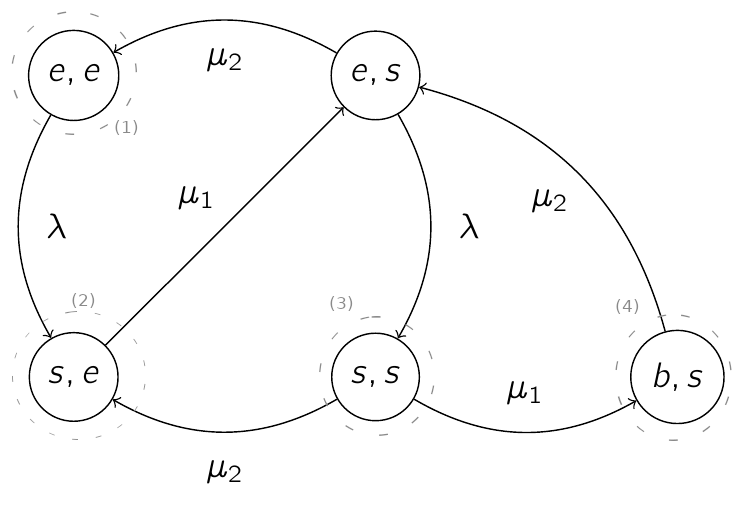
\includegraphics[width=0.65\textwidth]{pics/queue_nets_1_a.png}

\subsubsection*{b)}

stationary distribution $\rightarrow$ global balance equations:
\begin{align*}
\left(1\right)\lambda \cdot p\left(e,e\right)&=\mu _{2}\cdot p\left(e,s\right)\\
\left(2\right)\lambda \cdot p\left(e,e\right)+\mu _{2}\cdot p\left(s,s\right)&=\mu _{1}\cdot p\left(s,e\right)\\
\left(3\right)\lambda \cdot p\left(e,s\right)&=\left(\mu _{2}+\mu _{1}\right)\cdot p\left(s,s\right)\\
\left(4\right)\mu _{1}\cdot p\left(s,s\right)&=\mu _{2}\cdot p\left(b,s\right)
\end{align*}
normalization condition: $1=p\left(e,e\right)+p\left(s,e\right)+p\left(e,s\right)+p\left(s,s\right)+p\left(b,s\right)$
\begin{align*}
\cdots
\end{align*}
\begin{align*}
p ( e , e ) &= \frac { \mu _ { 1 } \mu _ { 2 } ^ { 2 } \left( \mu _ { 1 } + \mu _ { 2 } \right) } { \mu _ { 1 } \mu _ { 2 } ^ { 2 } \left( \mu _ { 1 } + \mu _ { 2 } \right) + \lambda \mu _ { 2 } \left( \mu _ { 1 } + \mu _ { 2 } \right) ^ { 2 } + \lambda ^ { 2 } \left( \mu _ { 1 } ^ { 2 } + \mu _ { 1 } \mu _ { 2 } + \mu _ { 2 } ^ { 2 } \right) }\\
p ( e , s ) &= \frac { \lambda \mu _ { 1 } \mu _ { 2 } \left( \mu _ { 1 } + \mu _ { 2 } \right) } { \mu _ { 1 } \mu _ { 2 } ^ { 2 } \left( \mu _ { 1 } + \mu _ { 2 } \right) + \lambda \mu _ { 2 } \left( \mu _ { 1 } + \mu _ { 2 } \right) ^ { 2 } + \lambda ^ { 2 } \left( \mu _ { 1 } ^ { 2 } + \mu _ { 1 } \mu _ { 2 } + \mu _ { 2 } ^ { 2 } \right) }\\
p ( s , s ) &= \frac { \lambda ^ { 2 } \mu _ { 1 } \mu _ { 2 } } { \mu _ { 1 } \mu _ { 2 } ^ { 2 } \left( \mu _ { 1 } + \mu _ { 2 } \right) + \lambda \mu _ { 2 } \left( \mu _ { 1 } + \mu _ { 2 } \right) ^ { 2 } + \lambda ^ { 2 } \left( \mu _ { 1 } ^ { 2 } + \mu _ { 1 } \mu _ { 2 } + \mu _ { 2 } ^ { 2 } \right) }\\
p ( s , e ) &= \frac { \lambda \mu _ { 2 } ^ { 2 } \left( \lambda + \mu _ { 1 } + \mu _ { 2 } \right) } { \mu _ { 1 } \mu _ { 2 } ^ { 2 } \left( \mu _ { 1 } + \mu _ { 2 } \right) + \lambda \mu _ { 2 } \left( \mu _ { 1 } + \mu _ { 2 } \right) ^ { 2 } + \lambda ^ { 2 } \left( \mu _ { 1 } ^ { 2 } + \mu _ { 1 } \mu _ { 2 } + \mu _ { 2 } ^ { 2 } \right) }\\
p ( b , s ) &= \frac { \lambda ^ { 2 } \mu _ { 1 } ^ { 2 } } { \mu _ { 1 } \mu _ { 2 } ^ { 2 } \left( \mu _ { 1 } + \mu _ { 2 } \right) + \lambda \mu _ { 2 } \left( \mu _ { 1 } + \mu _ { 2 } \right) ^ { 2 } + \lambda ^ { 2 } \left( \mu _ { 1 } ^ { 2 } + \mu _ { 1 } \mu _ { 2 } + \mu _ { 2 } ^ { 2 } \right) }
\end{align*}

\subsubsection*{c)}

\begin{align*}
E\left[S\right]&=1\cdot \left(p\left(s,e\right)+p\left(e,s\right)\right)+2\cdot \left(p\left(s,s\right)+p\left(b,s\right)\right)+0\cdot p\left(e,e\right)\\
E\left[S\right]&=\cdots\\
E [ S ] &= \frac { \lambda \left[ \lambda \left( 2 \mu _ { 1 } ^ { 2 } + 2 \mu _ { 1 } \mu _ { 2 } + \mu _ { 2 } ^ { 2 } \right) + \mu _ { 2 } \left( \mu _ { 1 } + \mu _ { 2 } \right) ^ { 2 } \right] } { \mu _ { 1 } \mu _ { 2 } ^ { 2 } \left( \mu _ { 1 } + \mu _ { 2 } \right) + \lambda \mu _ { 2 } \left( \mu _ { 1 } + \mu _ { 2 } \right) ^ { 2 } + \lambda ^ { 2 } \left( \mu _ { 1 } ^ { 2 } + \mu _ { 1 } \mu _ { 2 } + \mu _ { 2 } ^ { 2 } \right) }
\end{align*}

\subsubsection*{d)}
$p\left(e,e\right)+p\left(e,s\right)$ = proportion of time arrival can
actually occur = when 1st node is empty(e)
\begin{align*}
\lambda _{eff}&=\lambda \cdot \left(p\left(e,e\right)+p\left(e,s\right)\right)\\
\lambda _{eff}&=\cdots\\
\lambda _ {  eff } &= \frac { \lambda \mu _ { 1 } \mu _ { 2 } \left( \lambda + \mu _ { 2 } \right) \left( \mu _ { 1 } + \mu _ { 2 } \right) } { \mu _ { 1 } \mu _ { 2 } ^ { 2 } \left( \mu _ { 1 } + \mu _ { 2 } \right) + \lambda \mu _ { 2 } \left( \mu _ { 1 } + \mu _ { 2 } \right) ^ { 2 } + \lambda ^ { 2 } \left( \mu _ { 1 } ^ { 2 } + \mu _ { 1 } \mu _ { 2 } + \mu _ { 2 } ^ { 2 } \right) }
\end{align*}

\pagebreak

\subsubsection*{e)}


\begin{align*}
p_{block} &= P[\text{admitted customer gets blocked}]
\end{align*}

blocking requires two conditions: 
\begin{itemize}
\item first server is empty on arrival and second server is serving
\item service of 1st node finishes before 2nd node
\end{itemize}

\begin{align*}
p_{block} &= P[(e,s) \text{ on arrival x 1st service finishes before 2nd } | \text{ customer is admitted }]\\
&= P[(e,s) \text{ on arrival \textbar customer is admitted} ] \cdot P[\text{1st service finishes before 2nd}]\\ 
&= \frac{p\left(e,s\right)}{p\left(e,e\right)+p\left(e,s\right)}\cdot \frac{\mu _{1}}{\mu _{1}+\mu _{2}}\\
&= \frac { \lambda \mu _ { 1 } } { \left( \lambda + \mu _ { 2 } \right) \left( \mu _ { 1 } + \mu _ { 2 } \right) }
\end{align*}

\subsubsection*{f)}

\begin{align*}
E\left[D\right]&=\frac{E\left[S\right]}{\lambda _{eff}}&& \text{-  little's law -}\\
&=\ldots \\
&=\frac{\left(\lambda +\mu _{2}\right)\left(\mu _{1}+\mu _{2}\right)^{2}+\lambda \cdot \left(\mu _{1}\right)^{2}}{\mu _{1}\cdot \mu _{2}\cdot \left(\lambda +\mu _{2}\right)\left(\mu _{1}+\mu _{2}\right)}\\
&=\frac{1}{\mu _{1}}\cdot \mu _{2}+p_{block}\cdot \frac{1}{\mu _{2}}
\end{align*}


\subsection*{2.}

we solve without allowing use of reversibility property otherwise Burke's theorem
would immediately lead to the solution.

\begin{itemize}
\item  $T$: distribution of time between departures
\item  $s_{1}$: system content just before departure
\item  $s_{1}-1$: system content just after departure
\item  $d_{0}=Pr\left[s_{1}-1=0\right]$
\item  $1-d_{0}=Pr\left[s_{1}-1> 0\right]$
\end{itemize}

\begin{itemize}
\item  (i) $s-1> 0\rightarrow T\sim Exp \left(|\mu\right)$
\item  (ii) $s-1=0\rightarrow T\approx Exp \left(|\lambda\right)+Exp \left(|\mu\right)$
\end{itemize}

\begin{align*}
T^{\ast}\left(s\right)&=E\left[e^{{-sT}}\right]=E\left[E\left[e^{{-sT}}|s_{1}-1\right]\right]\\
&=E\left[e^{{-sT}}|s_{1}-1=0\right]\cdot d_{0}+E\left[e^{{-sT}}|s_{1}-1> 0\right]\cdot \left(1-d_{0}\right)\\
&=d_{0}\cdot \frac{\lambda }{\lambda +s}\cdot \frac{\mu }{\mu +s}+\left(1-d_{0}\right)\cdot \frac{\mu }{\mu +s}
\end{align*}

We know from 3.14: system content after departure $\sim $ system content at arrival instants

through PASTA we know: $d_{0}=1-\rho ,\rho =\frac{\lambda }{\mu }$

\begin{align*}
T^{{\ast }}\left(s\right)&=\frac{\lambda }{\lambda +s}\implies T\sim Exp \left(\ldots |\lambda \right)&& \text{-  $\rightarrow$ same as with Burke -}
\end{align*}

\subsection*{3.}

\subsubsection*{a)}

Define $S_i$ as nr of customers in node $i, i=1,2$. Then $(S_1, S_2)$ is a CTMC with state space $\mathbb{N} \times \mathbb{N}$ and state transition diagram:

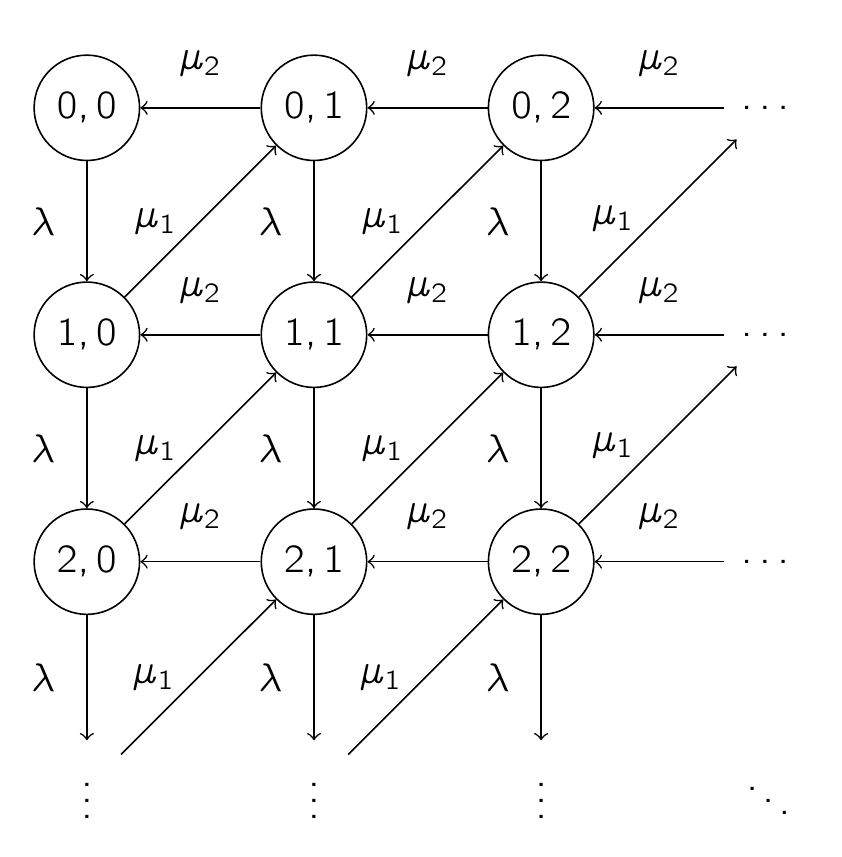
\includegraphics[width=0.65\textwidth]{pics/state_trans_que_nets_3.png}

\subsubsection*{b)}

\begin{align*}
\lambda s ( 0,0 ) &= \mu _ { 2 } s ( 0,1 )\\
\left( \lambda + \mu _ { 1 } \right) s \left( n _ { 1 } , 0 \right) &= \lambda s \left( n _ { 1 } - 1,0 \right) + \mu _ { 2 } s \left( n _ { 1 } , 1 \right)\\
\left( \lambda + \mu _ { 2 } \right) s \left( 0 , n _ { 2 } \right) &= \mu _ { 1 } s \left( 1 , n _ { 2 } - 1 \right) + \mu _ { 2 } s \left( 0 , n _ { 2 } + 1 \right)\\
\left( \lambda + \mu _ { 1 } + \mu _ { 2 } \right) s \left( n _ { 1 } , n _ { 2 } \right) &= \lambda s \left( n _ { 1 } - 1 , n _ { 2 } \right) + \mu _ { 1 } s \left( n _ { 1 } + 1 , n _ { 2 } - 1 \right) + \mu _ { 2 } s \left( n _ { 1 } , n _ { 2 } + 1 \right)
\end{align*}

\subsection*{4.}

\textbf{used formulas}

\begin{itemize}
\item  M/M/1 with arrival rate $\lambda $, service rate $\mu $
\item  $Pr\left[s=n\right]=\left(1-\rho \right)\rho ^{n}$ with $\rho =\frac{\lambda }{\mu }$, $n=0,1,2\ldots$ 
\item $E\left[S\right]=\frac{\lambda }{\mu -\lambda }=\frac{\rho }{\rho -1}$
\end{itemize}

\textbf{solution}

\subsubsection*{ a) }

stability condition for Jackson network: $\lambda \le \mu $
$\implies $ for our network: $2\cdot \lambda < \mu _{1}+\mu _{2}$  $\implies $ $\lambda _{1}=\lambda _{2}=\lambda $
$\implies $ Burke's theorem

\subsubsection*{ b) }

$E\left[D\right]=\frac{E\left[S\right]}{\lambda }$ little's law

we have a feedforward network:
\begin{align*}
E\left[S\right]&=E\left[S_{1}+S_{2}\right]\\
&=\sum _{{n_{1},n_{2}}}\left(n_{1}+n_{2}\right)\cdot Pr\left[S_{1}=n_{1},S_{2}=n_{2}\right]\\
&=\sum _{{n_{1},n_{2}}}\left(n_{1}+n_{2}\right)\cdot Pr\left[S_{1}=n_{1}\right]\cdot Pr\left[S_{2}=n_{2}\right]\\
&=E\left[S_{1}\right]+E\left[S_{2}\right]&& \text{-  because Jackson Network -}\\
&=\frac{\lambda }{\mu _{1}-\lambda }+\frac{\lambda }{\mu _{2}-\lambda }\\
&=\frac{\lambda }{\mu _{1}-\lambda }+\frac{\lambda }{\left(\mu -\mu _{1}\right)-\lambda }
\end{align*}

We minimize E[S], through Little's law this results in a minimal E[D]:

\begin{align*}
\frac{d}{d\mu _{1}}E\left[S\right]&=\frac{d}{d\mu _{1}}\left[\frac{\lambda }{\lambda -\mu _{1}}+\frac{\lambda }{\mu -\mu _{1}-\lambda }\right]=0\\
\frac{d}{d\mu _{1}}E\left[D\right]&=\frac{d}{d\mu _{1}}\left[\frac{\lambda }{\lambda -\mu _{1}}+\frac{\lambda }{\mu -\mu _{1}-\lambda }\right]=0\\
\Leftrightarrow \mu _{1}&=\frac{\mu }{2}
\end{align*}
\begin{align*}
\mu _{{1opt}}&=\frac{\mu }{2} && \mu_{1opt} \text{ in } ] \lambda, \mu - \lambda[\\ 
\mu _{{2opt}}&=\mu -\frac{\mu }{2}=\frac{\mu }{2}
\end{align*}
stability condition: $\lambda < \mu _{1}$

\subsubsection*{c)}

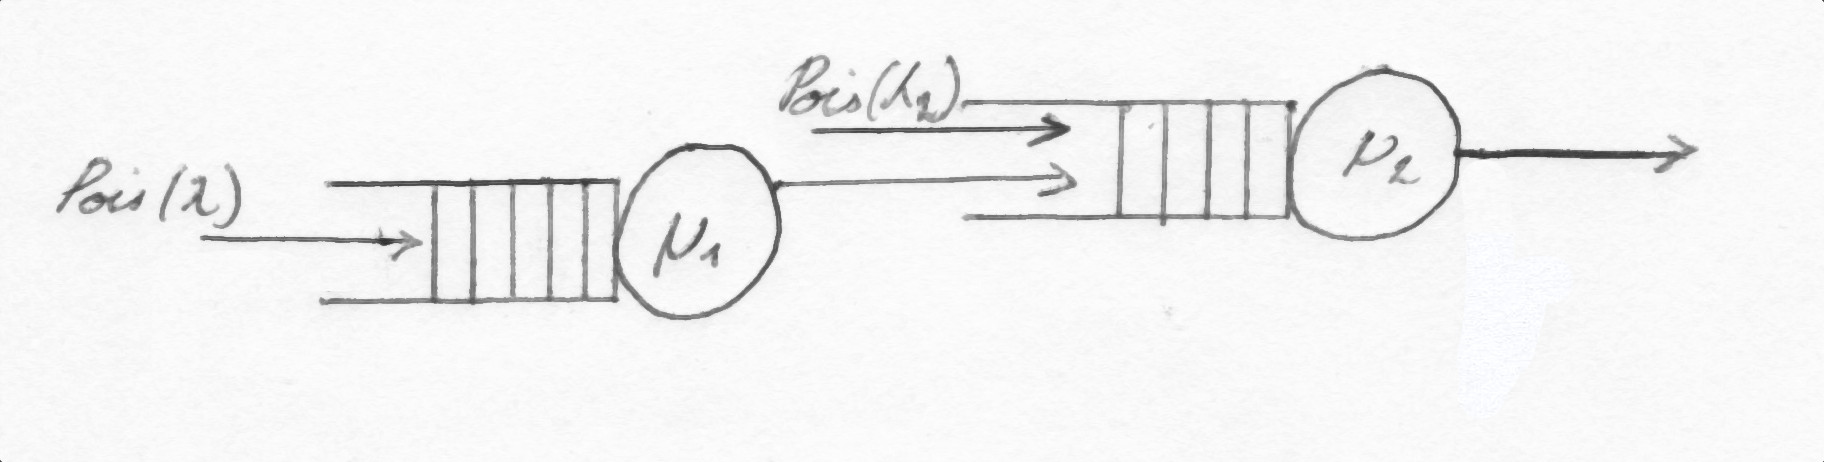
\includegraphics[width=0.75\textwidth]{pics/Ex09_jackson_net_4c.jpg}

\begin{align*}
\mu _ { 1 } = \frac { \mu - \gamma } { 2 } = \lambda + \frac { \mu - 2 \lambda - \gamma } { 2 } && \text{ and } &&
\mu _ { 2 } = \frac { \mu + \gamma } { 2 } = \lambda + \gamma + \frac { \mu - 2 \lambda - \gamma } { 2 }
\end{align*}

\subsubsection*{d)}

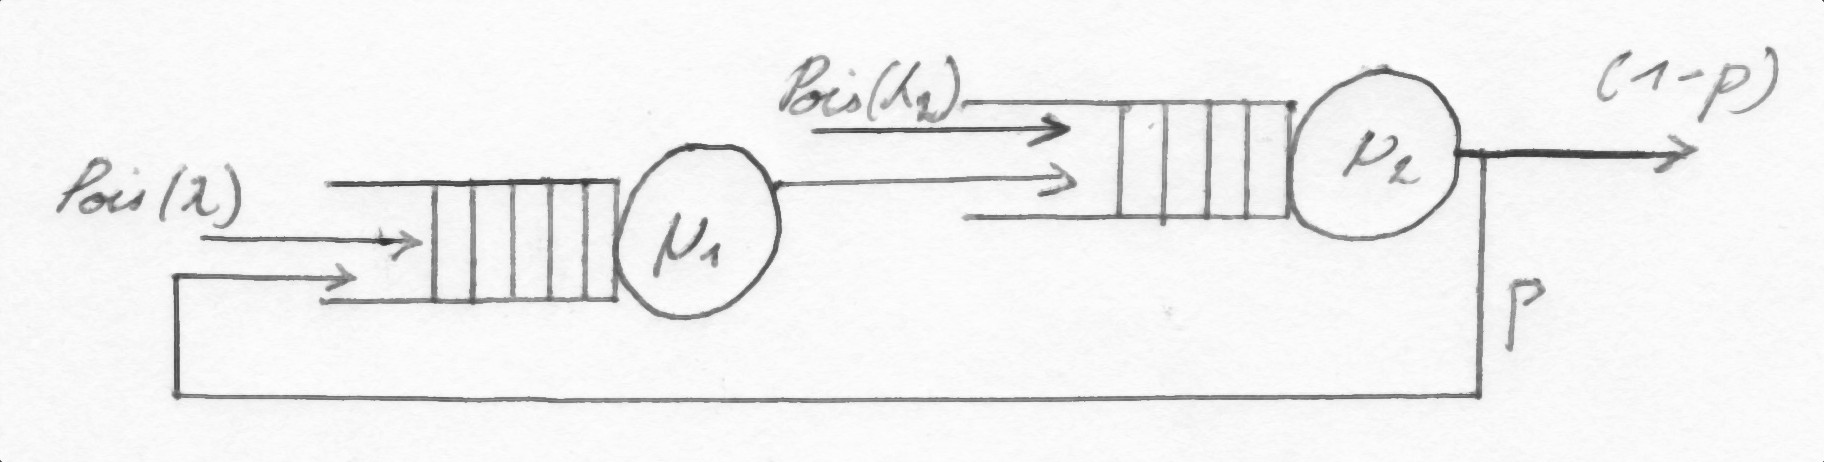
\includegraphics[width=0.75\textwidth]{pics/Ex09_jackson_net_4d.jpg}

traffic equations:
\begin{align*}
\lambda _{1}&=\lambda +p\cdot \lambda _{2}\\
\lambda _{2}&=\lambda _{1}+\gamma 
\end{align*}
\begin{align*}
\lambda _{1}&=\frac{\lambda +p\cdot \gamma }{1-p}\\
\lambda _{2}&=\frac{\lambda +\gamma }{1-p}
\end{align*}
as before we solve $\frac{dE\left[S\right]}{d\mu _{1}}=0$ for $\mu _{1} \ldots$

The constraint now becomes:

\begin{align*}
\mu > \frac { 2 \lambda + ( 1 + p ) \gamma } { 1 - p }
\end{align*}

The optimal distribution of the total service rate $\mu$ in this case is:

\begin{align*}
\mu _ { 1 } = \frac { \lambda + p \gamma } { 1 - p } + \frac { ( 1 - p ) \mu - 2 \lambda - ( 1 + p ) \gamma } { 2 ( 1 - p ) } && \text{ and } && \mu _ { 2 } = \frac { \lambda + \gamma } { 1 - p } + \frac { ( 1 - p ) \mu - 2 \lambda - ( 1 + p ) \gamma } { 2 ( 1 - p ) }
\end{align*}

\subsection*{5.}

\subsubsection*{a)}

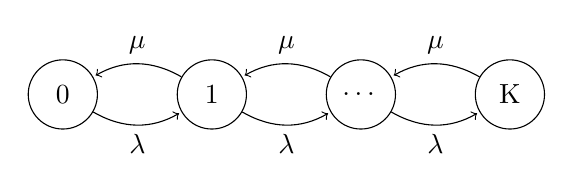
\begin{tikzpicture}
        \node[state]             (0) {0};
        \node[state, right=of 0] (1) {1};
        \node[state, right=of 1] (2) {\ldots};
        \node[state, right=of 2] (3) {K};

        \draw[every loop]
            (0) edge[bend right, auto=right]  node {$\lambda$} (1)
            (1) edge[bend right, auto=right] node {$\mu$} (0)
            (1) edge[bend right, auto=right]  node {$\lambda$} (2)
            (2) edge[bend right, auto=right]  node {$\mu$} (1)
            (2) edge[bend right, auto=right] node {$\lambda$} (3)
            (3) edge[bend right, auto=right]  node {$\mu$} (2)
            ;
\end{tikzpicture}

Local balance equation:

\begin{align*}
\lambda s ( n ) = \mu \cdot s ( n + 1 ) && n=0,\ldots, K-1
\end{align*}

A (normalized) solution for these balance equations can be found. Therefore—see (CN: Sec-
tion 2.2, p. 6.6)—the CTMC is reversible.

\subsubsection*{b)}

Burke's theorem states that when a queue is reversible the arrival process must correspond to the departure process.
The arrival process is not poisson because customers get discarded if K customers are in the queue $\Rightarrow$ finite capacity.


\section{ Simulation }

\subsection*{ 1. }

inversion method: calculate cdf by integrating density and invert this cdf.

Calculate the cumulative distribution function F(x) $\rightarrow $ integrate f(x):
\begin{align*}
F\left(x\right)&=\begin{cases}
x^{3}&0\le x\le 1\\
1&x> 1\\
\end{cases}
\end{align*}

inverse function: instead of returning y from x, the inverse function returns x given y: $F^{{-1}}\left(u\right)=\sqrt[3]{u}$ with $u=$ random sample $\in \left[0,1\right]$

\subsection*{ 2. }

\textbf{definitions}

\begin{itemize}
\item  $I_{0}\left(\kappa \right)=$ modified Bessel function of order 0
\item  $\kappa > 0$
\item  density von Mises Distribution: $f\left(x\right)=\frac{e^{{\kappa \cos \left(x\right)}}}{2\pi I_{0}\left(\kappa \right)}$ for $-\pi \le x\le \pi $, density is 0 otherwise
\end{itemize}

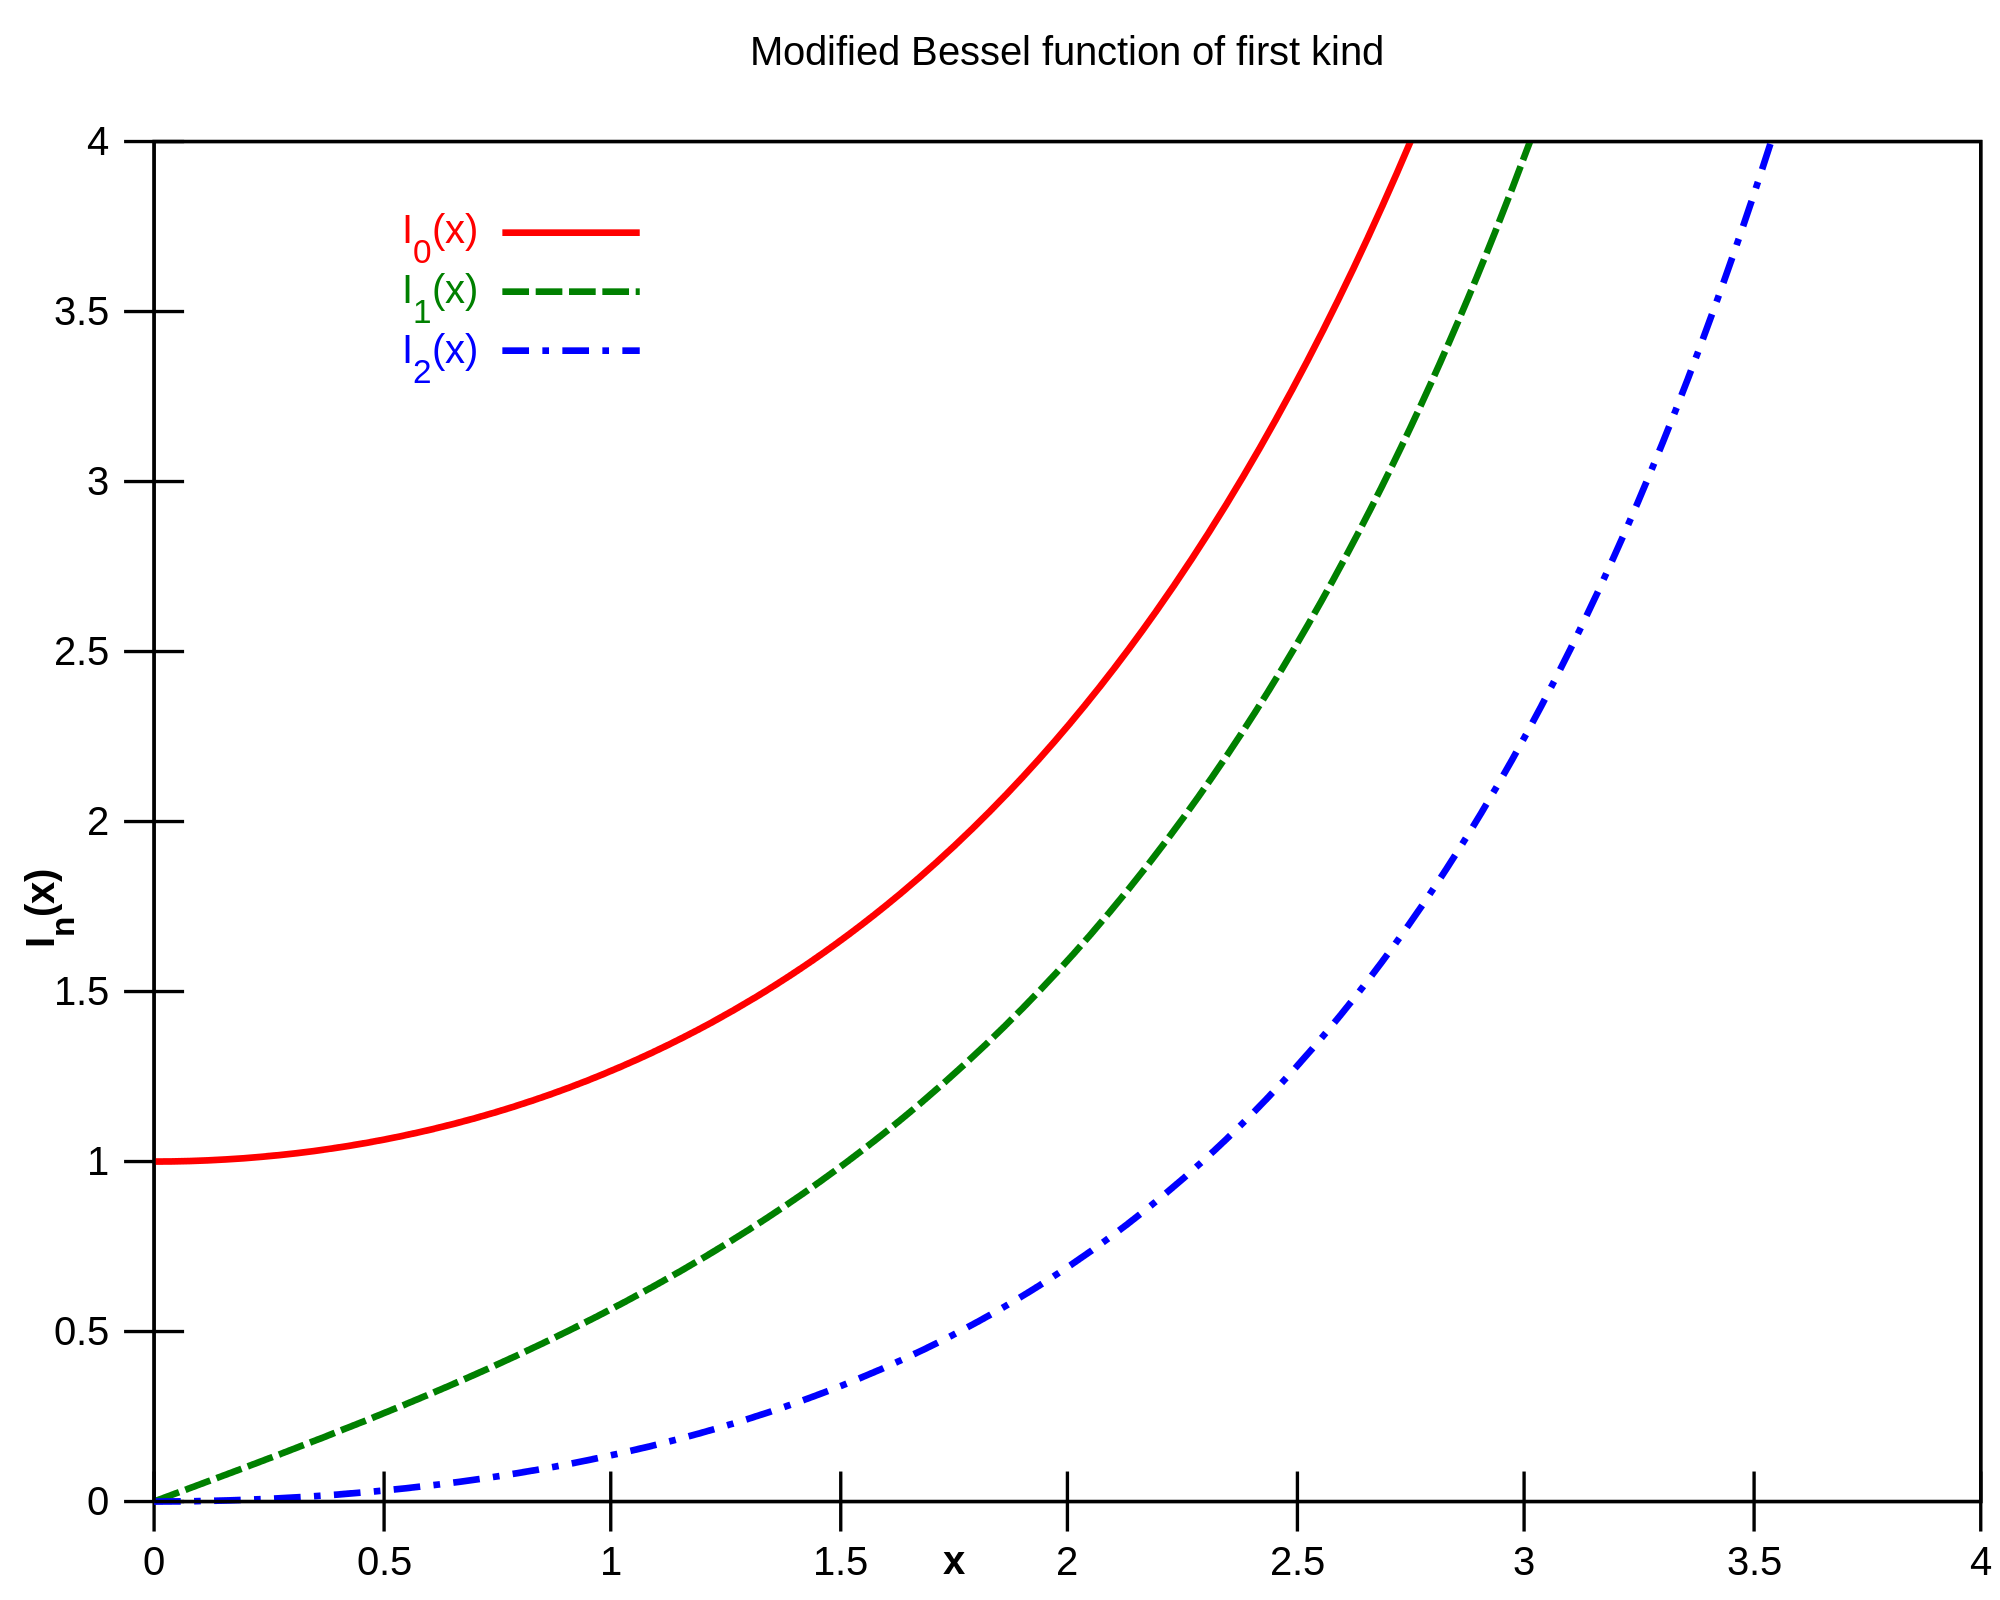
\includegraphics[width=0.65\textwidth]{pics/simulation_2_bessel.png}

\subsubsection*{ (1) }

based on plot: $I_{0}\left(\kappa \right)> 1$
finding extremum $\rightarrow $ derivative:

\begin{align*}
\frac{-K \sin \left(x\right)e^{{\kappa \cos \left(x\right)}}}{2\pi I_{0}\left(\kappa \right)}
\end{align*}
fill in for K=1, since we just want to know the sign: slope is positive for $f'(x)<0$,
0 for $f'(x)=0$ and negative for $f'(x)>0$, hence the maximum is at 0 when $-\pi \le x\le \pi $.

\subsubsection*{ (2) }

\begin{itemize}
\item  find $f_{y}$ such that $f_{y}\sim f_{x}$
\item  find $C\in \mathbb{R}> t$
\item  $C f_{y}\left(x\right)\ge f_{x}\left(x\right), \forall x\in \mathbb{R}$
\item  sample $u$ and $y\rightarrow $ if $u\left(f_{y}\left(y\right)\le f_{x}\left(y\right)\right)$ return y else sample again
\end{itemize}

\begin{align*}
f_{y}\left(y\right)&=\begin{cases}
\frac{\pi }{2}&-\pi < y\le \pi \\
0&otherwise\\
\end{cases}
\end{align*}

\begin{align*}
C = f(0) 2 \pi = \frac{e^{\kappa}}{I_0 (\kappa)}
\end{align*}

\subsection*{ 3 }

\subsubsection*{ (1) }

$F^{-1}(u) = (1-(1-u)^{1/b})^{1/a}$

\subsubsection*{ (2) }

$B\sim Beta\left(|\alpha ,\beta \right)$
\begin{align*}
Pr\left[B^{{\frac{1}{a}}}\le x\right]&=Pr\left[K\le x\right]\\
&=Pr\left[B\le x^{a}\right]\\
&=F_{B}\left(x^{a}\right)\\
&=\int _{0}^{{x^{a}}}f_{B}\left(t\right)dt\\
&=\int _{0}^{x}f_{B}\left(S^{a}\right)as^{{a-1}}ds&& \text{- clean int limits$\rightarrow$  substitute $t$ with $S^{a},a\in \mathbb{N}$ -}\\
&=\int _{0}^{x}\frac{1}{B\left(\alpha ,\beta \right)}\left(1-S^{a}\right)^{{\beta -1}}as^{{\alpha -1}}ds&& \text{-  solve $f_B(S^a)$, $\left(1-S^{a}\right)^{{\beta -1}}as^{{\alpha -1}}\approx f_{K}\left(s\right)$ -}\\
&=Pr\left[K\le x\right]\\
&=F_{k}\left(x\right)
\end{align*}

\subsubsection*{ (3) }

\begin{itemize}
\item  uniform random variable: $u\in \left[0,1\right]$
\item  $x_{K}=\left(1-\left(1-u\right)^{{\frac{1}{b}}}\right)^{{\frac{1}{a}}}$
\item $x_{B}=x^{a}_{K}=\left(1-\left(1-K\right)^{{\frac{1}{b}}}\right) \rightarrow $ given: $\alpha = 1$
\end{itemize}

\subsection*{ 4. }

\begin{align*}
J&=\int _{0}^{1}\int _{0}^{1}e^{\left(x+y\right)^{2}}dydx\\
&=E\left[e\left(x+y\right)^{2}\right]&& \text{-  double integral is like expectation, $x,y\sim $ uniform [0,1] -}\\
&=\int _{0}^{1}\int _{0}^{1}e^{\left(x+y\right)^{2}}f_{x}\left(x\right)f_{y}\left(y\right)dxdy\\
J_{K}&=\frac{1}{K}\sum _{{i=1}}^{K}e^{\left(x_{i}+y_{i}\right)^{2}}
\end{align*}
monte carlo $\rightarrow x_{1},\ldots ,x_{K}y_{1},\ldots ,y_{K}$ generate samples from uniform intervals 
correlation $\left(y_{i,}1-y_{i}\right)< 0$

\begin{align*}
\widehat{J}_{K}&=\frac{1}{K}\sum _{{i=1}}^{K}\frac{1}{2}e^{\left(x_{i}+y_{i}\right)^{2}}+e^{\left(2-x_{i}-y_{i}\right)^{2}}
\end{align*}

negative correlation antithetic $\rightarrow $ see syllabus $\rightarrow $ smaller amount of samples for same conf variables

\subsection*{ 5. }

samples $Z_{1},\ldots ,Z_{K}$

\begin{align*}
\widehat{J}_{K}&=\frac{1}{K}\sum _{i}=1^{K}Z_{i}^{3}e^{{Z_{i}}}&& \text{-  corr(Z, -Z) = E([Z-E(Z)][-Z-E(-Z)]) = -1 -}\\
\widehat{J}_{K}^{a}&=\frac{1}{K}\sum ^{K}\frac{1}{2}\left(Z^{3}_{i}e^{{Z_{i}}}-Z_{i}^{3}e^{{-Z_{i}}}\right)
\end{align*}
monotone, negative correlation $\rightarrow $ lower variance

\subsection*{ 6. }

u is uniformly distributed, $\widetilde{u} = 1-u$ is uniformly distributed. $F_{x}\left(x\right)=1-e^{{-x}}$\\
$x\rightarrow \widetilde{u}=e^{-x}\rightarrow u=1-e^{-x}\rightarrow -\ln \left(1-e^{-x}\right)$\\
$\exp \rightarrow uniform\rightarrow uniform\rightarrow \exp $\\
$corr\left(\widetilde{u},u\right)< 0-\ln \left(\right)\rightarrow corr\left(-\ln \left(\left(\widetilde{u}\right),-\ln \left(u\right)\right)\right)< 0\rightarrow corr\left(x,-\ln \left(1-e^{-x}\right)\right)< 0$

\subsection*{ 7. }

\subsubsection*{ (1) }

\begin{align*}
\prod _{{\{x+y\le t\}}}\left(x+y\right)&=\begin{cases}
1&x+y< t\\
0&x+y> t\\
\end{cases}
\end{align*}
\begin{align*}
Pr\left[x+y\le t\right]&=E\left[\prod _{{\{\}}}\left(x+y\right)\right]
\end{align*}
\begin{align*}
\widehat{J}_{K}&=\frac{1}{K}\sum _{{i=1}}^{K}\prod _{{\{\}}}\left(x_{i}+y_{i}\right)
\end{align*}

\subsubsection*{ (2) }

\textbf{definitions}

\begin{itemize}
\item  $h$ is the indicator function
\item  we leave the {} out the subsript of $\prod _{{\{\}}}$ for clarity
\end{itemize}

\textbf{solution}

\begin{align*}
\widehat{J}_{K}^{{cond}}&=E\left[\prod ^{{\ast }}\left(X+Y\right)\right]\\
&=E\left[E\left[\prod ^{{\ast }}\left(X+Y\right)|X\right]\right]\\
&=E\left[\prod _{{X+Y\le t}}\left(X+Y\right)|X\right]\\
&=E\left[\prod _{{y\le t-x}}\left(Y\right)|X\right]\\
&=G\left(t-x\right)\\
&=Pr\left[y\le t-X|X\right]
\end{align*}
\begin{align*}
J&=E\left[\prod ^{{\ast }}\left(X+Y\right)\right]=E\left[G\left(t-x\right)\right]\\
\widehat{J}_{K}^{{cond}}&=\frac{1}{K}\sum _{{i=1}}^{K}G\left(t-x_{i}\right)&& \text{-  better because only one variable to sample -}
\end{align*}

\subsubsection*{ (3) }

\textbf{definitions}

\begin{itemize}
\item  $u,E\left[h\left(u\right),V,g\left(V\right),E\left(g\left(V\right)\right)\right]$
\end{itemize}

\textbf{solution}

\begin{align*}
E\left[h\left(u\right)\right]&=E\left[h\left(u\right)+\left[g\left(V\right)-E\left(g|V\right)\right]\right]K&& \text{-  $K\in \mathbb{R}$ -}\\
E\left[G\left(t-X\right)\right]&=E\left[G\left(t-X\right)+K\left[X-\mu _{x}\right]\right]&& \text{-  determine K online -}
\end{align*}
\begin{align*}
\widehat{J}_{K}&=\frac{1}{K}\sum _{{i=1}}^{K}\left(G\left(t-x_{t}\right)+K\left(x_{i}-\mu _{x}\right)\right)
\end{align*}

\pagebreak


\end{document}
